\input{präambel.tex}	% all latex init code here!

% !TEX root = dokumentation.tex

\newacronym{IDE}{IDE}{Integrated Development Environment}
\newacronym{RPG}{RPG}{Role Play Game}
		% abkürzungen hier rein

\begin{document}
% !TEX root = dokumentation.tex
\begin{titlepage}

	\obeylines
	\begin{center}
		
\includegraphics[width=0.5\textwidth,height=!]{img/dhbw.pdf}\\ [0.5cm]
		{\huge\bfseries{} Konzeption und Entwicklung\\ eines educational games}
		{\Large{}spielerisch Schulwissen vermitteln auf Android}\\ [1.6cm]
		{\large \textbf{Studienarbeit T2\_3100}}\\ [1.6cm]
		{des Studiengangs Angewandte Informatik}
		{an der Dualen Hochschule Baden-Württemberg Karlsruhe}

		{von} \\ [0.5cm]
		{\large \bfseries \textbf{Marc Mahler \& Marvin Zerulla}} \\ [0.666cm]
		{\large Datum der Fertigstellung \today}
	\end{center}

	\vfill

	\begin{tabular}{l@{\hspace{2cm}}l}
		\textbf{Bearbeitungszeitraum}		& 24 Wochen \\
		\textbf{Matrikelnummern}			& 8513588 -- 5782186 \\
		\textbf{Kurs}						& TINF14B2 \\
		\textbf{Ausbildungsfirmen}			& Fiducia \& GAD - 1\&1 \\
		\textbf{Betreuer der DHBW}			& Prof. PhD. Kay Margarethe Berkling
	\end{tabular}

\end{titlepage}

%% !TEX root = dokumentation.tex
\obeylines
\pagenumbering{roman}
\section*{Erklärung}\vspace*{2em}
% Seite 8
% http://studium.ba-bw.de/fileadmin/media/allgemein/bestimmungen/btechnik/richtlinien/Richtlinien_Praxismodule_Studien_und_Bachelorarbeiten_2011.pdf
Gemäß § 5 (3) der \enquote{Studien- und Prüfungsordnung DHBW Technik} vom 29.9.2015
Hiermit erklären wir,
\begin{enumerate}
	\item{ dass wir die vorliegende Arbeit selbstständig verfasst und keine anderen als die angegebenen Quellen und Hilfsmittel verwendet haben. }
	\item{ dass die Übernahme von Zitaten und Gedankengut anderer Autoren gekennzeichnet wurde. }
	\item{ dass die eingereichte elektronische Fassung exakt mit der Schriftlichen übereinstimmt. }
	\item{ dass wir die Studienarbeit keiner externen Prüfung vorgelegt haben. }
\end{enumerate}\vspace{3em}

\begin{tabular}{lp{2em}l}
	Karlsruhe, den \today  && \hspace{7cm} \\\cline{1-1}\cline{3-3}
	Ort, Datum     &&  Marc Mahler,\hfill Marvin Zerulla
\end{tabular}
\newpage

%% !TEX root = dokumentation.tex
\section*{Abstract}
Dass Lernspiele funktionieren ist mittlerweile eine akzeptierte Ansicht. Dennoch fehlen professionell umgesetzte Lernspiele, welche die komplette Bandbreite an Wissen vermitteln. Eine Kombination aus vielen Lernspielen könnte dies erreichen und so eine Schulausbildung erweitern bzw. teilweise ersetzen.
Diese Arbeit handelt von der Entwicklung eines Lernspieles, dabei werden Konzepte der Gamification, Personas, Psychologie und Game Design generell verwendet. Für die Arbeit wurden gängige Lernmethoden, als auch klassische Videospiele analysiert. Das Spiel wird konzipiert, entwickelt und über die Entwicklung hinweg bereits kontinuierlich evaluiert. Der Spielspaß steht dabei im Vordergrund der Entwicklung.
Ergebnis der Arbeit ist ein Rennspiel für Android. Das Spiel unterstützt beliebige Lernmaterialien, eignet sich aber vor allem für schnell abrufbares Faktenwissen.

\vfill

\section*{Abstract}
That learning games work is now an accepted view. However, there is still a lack of professionally implemented learning games which can provide the complete range of knowledge and thus possibly replace a school education.
This work deals with the development of a learning game, in which concepts of gamification, personas, psychology and game design are generally used. For the work, common learning methods as well as classical video game were analyzed. The game is designed, developed and continuously evaluated over the development. The game is the focus of the development.
Result of the work is a racing game for Android. The game supports any learning materials, but is suitable for fast-retrievable factual knowledge.

\vfill\vfill\newpage


\pagestyle{empty}
\begin{singlespace}
	\microtypesetup{protrusion=false}
	\tableofcontents{}	\addtocontents{toc}{~\hfill\textbf{Seite}\par}\pagebreak
	\listoffigures{}	\addtocontents{lof}{~\hfill\textbf{Seite}\par}
	\listoftables{}		\addtocontents{lot}{~\hfill\textbf{Seite}\par}
	\pagebreak
	\microtypesetup{protrusion=true}
	\printglossary[type=acronym,title={Abkürtzungen}]
	\pagebreak
\end{singlespace}

\pagestyle{scrheadings} 	%starting from here cool headings
\setcounter{page}{1}
% !TEX root = dokumentation.tex
\section{Einleitung}
	Üblicherweise geht es in der Spieleentwicklung darum, dem Spieler eine bestimmte Emotion zu vermitteln, meistens ist dies Spaß oder Freude.\footcite[Abstract]{persona} Soziologen und Lehrer <TODO:Quelle? und genauer> hatten die Idee, dass durch Spiele auch Wissen vermittelt werden kann. Wenn diese Lernspiele betrachtet werden, fällt oft auf, dass der Spielspaß dabei vernachlässigt wurde (siehe \ref{sssec:lernspielanalyse}).

	Kinder zeigen in einem gewissen Alter eine Abneigung gegen Schule und die Vermutung, dass dies am Zwang liegt, kommt auf<TODO:Quelle?>. Übertragen auf Lernspiele ist die These: wenn das Spiel stetig zum Lernen auffordert, aber keinen Gegenwert bringt, wird dem Spiel auch mit Abneigung begegnet.
	Hier bleibt die Frage stehen, ob lernen nicht effektiver wird, wenn das Spiel auch Spaß macht.

	Durch das spielerische Lernen können die Spieler Fähigkeiten schulen oder etwas für das Leben lernen, während sie Spaß am Spiel haben. Können die Lerninhalte erfolgreich mit dem Spielspaß kombiniert werden, merkt der Spieler unter Umständen nicht einmal, dass gerade Wissen vermittelt wird.

	Das Ziel dieser Studienarbeit ist die Entwicklung eines Lernspiels für Android. Die Problemstellung liegt dabei darin, sowohl den Spielspaß, als auch den Lernerfolg zu vermitteln. Das erwartete Ergebnis ist zum einen die Veröffentlichung des Spiels sowie die Erarbeitung und Anwendung von Wissen über Spieleentwicklung, Gamification und Game-Engines. <TODO:evaluation und playtests erwähnen>

\subsection{Aufgabenstellung}
	Folgende Anforderungen konnten für die Durchführung der Studienarbeit und die Entwicklung der Software definiert werden:
	\begin{itemize}
		\item{ Die Zielgruppe für das Lernspiel besteht aus Kindern im Alter der ersten bis sechsten Klasse.\footnote{Nach deutschem Schulsystem, also Kinder von circa 6 bis 12 Jahren.} Nach Möglichkeit soll dieses Spiel und die zugehörige Lernplattform auch Flüchtlingskindern zur Verfügung gestellt werden. }
		\item{ Das Spiel soll Android als Zielplattform unterstützen. Dort befindet sich im mobilen Bereich die größte Nutzerbasis. (siehe \ref{ssec:android}) }
		\item{ Es besteht keine Notwendigkeit der Einhaltung der Lernstandards. Die Spieler (Kinder) sollen mit dem Spiel Spaß haben und das Spiel auch spielen \enquote{wollen}.\footnote{<TODO: mit Berkling absprechen>} }
		\item{ Als Beispiel wurde \url{https://arcademics.com} genannt, eine Seite welche Spiele der gewünschten Art beinhaltet. }
		\item{ Das Spiel soll teil der Lernplattform von Prof. PhD. Kay Berkling werden und Lernerfolge an diese melden. }
		\item{ Das Spiel soll auch offline spielbar sein. Falls Lernerfolge anfallen sollen diese nachträglich an die Lernplattform gemeldet werden. }
		\item{ Der Spaß steht im Vordergrund und die Lernerfolge sollen unterbewusst stattfinden. }
	\end{itemize}
	Für die Umsetzung der Lerninhalte ist somit ein geeignetes Format zu wählen, welches den Spielspaß nicht mindert und dennoch wichtige Grundfertigkeiten vermittelt.
	Bei der Auswahl der Gamification-Modelle gilt besondere Achtsamkeit bei der Anfälligkeit der Zielgruppe gegenüber den gewählten Methoden. Somit soll das Spiel sowohl die Aufmerksamkeit des Spielers erreichen, sowie diese für einen gesetzten Zeitraum halten.

\subsection{Spielidee}\label{ssec:spielidee}
	Um zur endgültigen Spielidee zu gelangen, wurden mehrere Ideen ausgearbeitet (siehe \ref{ssec:idee}) und gegen unsere Kriterien (siehe \ref{ssec:kriterien}) abgewogen.
	Als endgültige Spielidee wurde ein Rennspiel ausgearbeitet. In diesem mit verschiedenen Dingen (Beispielsweise: ein Würfel, ein Auto oder eine Rakete) ein Rennen stattfinden sollen. Um Lerninhalte in ein Rennspiel einzubauen wurden mehrere Möglichkeiten ausgearbeitet:
	\begin{itemize}
		\item{ Aufgabe zum Start des Rennens. Hier kann der schnellste Spieler als Erstes starten. Durch eine maximale Zeit und mehrere Versuche kann der Nachteil beschränkt werden, um schwächere Spieler besser zu inkludieren. }
		\item{ Aufgaben in Form von Weggabelungen (wie beispielsweise Tore oder Schanzen). Eine Aufgabe erscheint rechtzeitig\footnote{<TODO:Was in diesem Kontext rechtzeitig bedeutet wird noch definiert.>} vor der Gabelung auf dem Bildschirm. Bei jeder Abzweigungsmöglichkeit steht eine Lösung zur Aufgabe. Fährt ein Spieler falsch, bekommt er einen Nachteil oder alle Spieler die korrekt fahren einen Vorteil. }
		\item{ Learn-To-Win: Spieler können durch lösen von Aufgaben virtuelles Geld verdienen und gewisse Vorteile im Spiel durch Einsatz des Geldes genießen. Diese Idee ist von dem Pay-To-Win Monetarisierungsmodell abgeleitet. }
	\end{itemize}
	Ein wichtiges Kriterium für die Spielidee war, dass Lerninhalte ein Teil von dem Spiel sind und so auch das Lernen selbst durch Spaß angeregt wird.
	Das Spiel selbst soll in mindestens zwei Spielmodi spielbar sein:
	\begin{itemize}
		\item{ Online Multiplayer: Rennen fahren mit anderen echten Personen über das Internet. }
		\item{ Offline Zeitrennen: auf Strecken gegen die Zeit fahren. }
		\item{ Optional: Offline gegen Computer: wie das Onlinespiel nur mit Computergegnern. }
	\end{itemize}
	Auf grafischer Ebene soll das Spiel mit einer 3D Grafik entwickelt werden. Die Kamera Ansicht soll von leicht schräg oben dem Gefährt folgen.

\subsection{Abgrenzung}
	Das im Rahmen der Studienarbeit entwickelte Spiel wird im App-Store zur Verfügung stehen und in der Lernplattform von Prof. PhD. Kay Berkling integriert. Auf weitere Aspekte von Vermarktung und Vertrieb wird im Rahmen der Studienarbeit verzichtet.
	Im Bereich der Spieleentwicklung wird auf eine eigenständige Entwicklung von Charaktermodellen und Grafiken verzichtet. Diese werden über externe Quellen eingekauft und in die Anwendung integriert.

	Lernaufgaben werden nicht im Rahmen der Arbeit erstellt, Aufgaben sollen durch eine Schnittstelle geladen werden.

\subsection{Vorgehen}
	Auf Basis der Spielidee werden Play-Personas\footcite{persona} ausgearbeitet, danach ein Gamification-Modell\footnote{<TODO:warum Gamification? und wieso mit spielen kombinieren?>} auf diese Personas zugeschnitten. Das Gamification-Modell soll Spieler anregen das Spiel länger zu spielen und so mehr zu lernen. Der Fokus liegt dabei stark auf der Verbindung von Gamification und spielerischem Lernen.
	<TODO:Brainstorming erwähnen>
	Das Spiel soll in einer gängigen Game-Engine entwickelt werden. Um eine passende Game-Engine zu wählen, wird eine Evaluation durchgeführt (siehe \ref{ssec:engineeval}).
	Die Entwicklung des Spiels geschieht über anfängliches Prototyping und eine anschließenden Implementierung in der Game-Engine. Am Ende der Implementierung soll das entstandene Spiel in die bereits vorhandene Lernplattform von Prof. PhD. Kay Berkling eingegliedert und über diese vertrieben werden.

% !TEX root = dokumentation.tex
\section{Grundlagen}
	In diesem Kapitel werden die Theoretischen Grundlagen der Arbeit aufgezeigt.
\subsection{Android als Zielplattform erklären}
\subsection{Game-Engines}
	Eine Game-Engine soll die Entwicklung von Spielen erleichtern. Dies funktioniert in dem Entwicklern Arbeit abgenommen wird Beispielsweise in dem eine einfach zu nutzende Physik-Komponente oder ein \gls{IDE} bereitgestellt wird. Eine Game-Engine stellt oft verwendete Funktionen Spielentwicklern zu Verfügung und beschleunigt die Entwicklung.
	\subsubsection{Unity}
	\subsubsection{Unreal}
	\subsubsection{Cryengine}
	\subsubsection{mehr?}
\subsection{Persona}\label{ssec:persona}
	Ein Persona ist eine Technik aus dem UI Bereich wo durch imaginäre Nutzer (Personas) die Useability verbessert werden soll.
\subsection{Gamification}
	modell selbst machen leicht mit top games der zielgruppe und zielgruppenanalyse
	Psychologische Grundlagen für Spiele?
	Vorstellung und generelles pro contra
\subsection{Lernziele definition}

% !TEX root = dokumentation.tex
\section{Konzipierung}
Das folgende Kapitel beschäftigt sich mit der Konzipierung des Spiels ansich. Dabei werden zunächst die erarbeiteten und vorgegebenen Kriterien zusammengefasst, mehrere Spielideen anhand dieser Kriterien überprüft und anschließend eine finale Spielidee entwickelt. Im weiteren Verlauf des Kapitels werden Functional und non-functional Requirements erörtert und in Use-Cases unterteilt. Anhand dieser Requirements wird dann im Kapitel \ref{sec:impl} Implementierung das Spiel entwickelt. Weiterhin werden in diesem Kapitel die Spielregeln verfasst und weitere Elemente, wie die Steuerung oder computergesteuerte Gegner (e.g. Bots) betrachtet. Abschließend soll betrachtet werden, wie die im Grundlagenteil erfassten Lernziele in Verbindung mit dem Spiel umgesetzt werden können.
\subsection{Kriterien für die Spielidee}\label{ssec:kriterien}
	Auf Basis der in der Aufgabenstellung genannten Kriterien und mit Erweiterung durch eigens erarbeitete Kriterien konnte ein Kriterienkatalog entwickelt werden. Damit eine vollständige Zusammenfassung aller Kriterien möglich ist, werden die Kriterien aus der Aufgabenstellung erneut aufgegriffen.
	\begin{enumerate}
		\item{Das Spiel soll levelbasiert sein, d.h. dass voneinander unabhängige Spielabschnitte vorhanden sind.}
		\item{Der Umfang des Spiels ist auf zwei bis drei Stunden Spielspaß ausgelegt. Durch modulare Gestaltung (Levels) kann das Spiel im Nachhinein erweitert werden.}
		\item{Das Spiel ist ein \enquote{educational game}, der Spielspaß steht im Vordergrund. Die Spieler sollen unbewusst nebenbei lernen.}
		\item{Aus Punkt 3 folgt: das Lernen selbst soll Spaß machen. Dies soll erreicht werden indem Lernen ein fester Bestandteil des Spiels ist und nicht als Aufgabe, zu der die Spieler genötigt werden.}
		\item{Das Spiel soll \enquote{casual} sein, d.h. ein Spiel \enquote{für zwischendurch} sein.}
		\item{Der vollständige Programmieraufwand für das Spiel ist auf 3 Monate Arbeit ausgelegt. Somit bleiben weitere volle drei Monate für das Verfassen der Arbeit.}
		\item{Ziel ist, eine originelle Spielidee zu entwickeln, sodass das Spiel kein Klon eines bereits existierenden Spiels ist.}
		\item{Als Beispiele zur Orientierung wurde \enquote{arcademics.com} genannt, welche Spiele der gewünschten Art beinhaltet, jedoch eine Internetverbindung benötigt. Daraus ergibt sich, dass das Spiel auch offline spielbar sein soll.}
		\item{Bei frühen Brainstorming-Sessions konnte sich darauf geeinigt werden, dass das Spiel in keinem Fall ein \gls{RPG} sein soll.}
		\item{Es besteht keine Notwendigkeit der Einhaltung der Lernstandards. Die Spieler sollen mit dem Spiel Spaß haben und das Spiel auch spielen wollen.}
		\item{Die Zielgruppe für das Spiel ist durch die Persona aus Kapitel 2<TODO: richtige Verlinkung> gegeben. Nach Möglichkeit soll dieses Spiel und die zugehörige Lernplattform auch Flüchtlingskindern zur Verfügung gestellt werden.}
	\end{enumerate}

	Die Entstehung dieser Kriterien ist teilweise auf die Ergebnisse aus dem Brainstorming zurückzuführen. Durch das Brainstorming konnten die Erwartungen der Projektteilnehmer an das Spiel weiter spezifiziert werden. Somit ist eine genaue Trennung der Kriterien vom Brainstorming nur schwer möglich und dient lediglich der Übersichtlichkeit.

\subsection{Gamification Modell}
\subsection{Lernziele Definition}

\subsection{Brainstorming \& Game Design}\label{ssec:idee}
	Über mehrere Gespräche hinweg wurden Ideen für das zu entwickelnde Spiel gesammelt. Dieses Kapitel hat zum Zweck, den Abauf der Ideenfindung in eine Reihenfolge zu bringen und diese zu präsentieren.
	\begin{enumerate}
		\item{Chemie / Physik Simulation:}
		\begin{itemize}
			\item{Die Simulation findet in einer Laborumgebung statt. Dabei steuert der Spieler den Laborarbeiter (bzw. aus der Sicht des Labrarbeiters).}
			\item{Der Spieler führt einfache Experimente aus den Bereichen Chemie und Physik durch.}
			\item{Fehler, welche dem Spieler in den Experimenten passieren, führen zum Scheitern des Versuchs.}
			\item{Der Spieler hat die Möglichkeit, die Hände des Laborarbeiters zu steuern.}
			\item{Alternativ kann der Spieler über den Touchscreen mit den Utensilien im Labor interagieren.}
			\item{Die Idee wurde verworfen, da eine realistische Steuerung von Experimenten aus Chemie und Physik nur schwer über einen Touchscreen umzusetzen ist. Weiterhin ist die für diese art von Spiel benötigte Physiksimulation ungeeignet für die Zielplattform. Außerdem stellt diese Idee nicht den gewünschten Lernerfolg für die gewünschte Zielgruppe zur Verfügung. }
		\end{itemize}
		\item{Rätselspiel:}
		\begin{itemize}
			\item{Der Spieler soll eine Art Rätsel lösen welche automatisch in unterschiedlichen Schwierigkeitsgraden generiert werden kann.}
			\item{Die Idee wurde aufgrund eines fehlenden Rätselkonzepts, fehlender weiterer Ideen und großer einschränkung der Zielgruppe verworfen.}
		\end{itemize}
		\item{Simulation von Motoren und Getrieben:}
		\begin{itemize}
			\item{Vor Spielbeginn bekommt der Spieler eine Strecke angezeigt. Diese Strecke ist in 2D und zeichnet sich durch Höhenunterschiede aus.}
			\item{Der Spieler wählt auf Basis der Strecke aus einer Sammlung verschiedener Motoren den Besten aus. Beispielsweise ist ein 2-Takt Motor für steile Berge besser geeignet als ein 4-Takt Motor.}
			\item{Der Spieler bekommt mehrere Treibstoffe (Benzin, Diesel, \dots) zur Auswahl und kann entsprechend der Strecke und des Motors wählen.}
			\item{Während der Fahrt hat der Spieler die Möglichkeit, über Schaltflächen den ausgewählten Gang des Getriebes zu wechseln.}
			\item{Bei der Auswahl von Treibstoffen, Motoren und Gangschaltungen werden dem Spieler Informationstexte angezeigt und vorgelesen.}
			\item{Um das Level bzw. das Spiel abzuschließen, muss die Strecke in der vorgegebenen Zeit absolviert werden.}
			\item{Die Idee wurde nach dem Kickoff-Meeting vollständig verworfen, da die Umsetzung der Lernziele nicht in gewünschter Form möglich ist.}
		\end{itemize}
		\item{Rennfahrspiel Version 1:}
		\begin{itemize}
			\item{Der Spieler nimmt an einer wilden Renntour durch die Stadt teil.}
			\item{Der Spieler wird von der Polizei verfolgt und bekommt beim geschnappt werden verschiedene Annimationen des Scheiterns angezeigt.}
			\item{Sollte der Spieler scheitern, kann er eine Aufgabe absolvieren um einen weiteren Versuch zu erhalten. Das ist drei mal möglich.}
			\item{Diese Aufgaben / Minigames sind beispielsweise:}
			\begin{itemize}
				\item{Ampel: Der Spieler muss rechtzeitig reagieren um an einer roten Ampel anzuhalten.}
				\item{Polizei: Der Spieler muss die Anweisungen der Polizei rechtzeitig befolgen. Anweisungen können z.~B.\@ das \enquote{Rechts ranfahren}sein.}
				\item{Sprungschantze: Der Spieler benötigt die richtige Geschwindigkeit um den Sprung perfekt zu absolvieren.}
			\end{itemize}
			\item{Die Idee wurde nach dem Kickoff-Meeting vollständig verworfen, da die Umsetzung der Lernziele nicht in gewünschter Form möglich ist.}
		\end{itemize}
	\end{enumerate}
	Aus diesen Ideen und in Verbindung mit den Informationen aus dem Kickoff-Meeting konnte die finale Spielidee entwickelt werden. Dabei wurde die Idee eines Rennspiels beibehalten und so angepasst, dass eine Umsetzung der Lernziele gut umsetzbar ist.
	\begin{enumerate}
		\item{Das Rennspiel wird dem Spieler aus der \enquote{Top-Down}-Ansicht präsentiert. Dabei ist die Kamera leicht schräg auf die Rennstrecke gerichtet, sodass die Modelle der Fahrzeuge dreidimensional sind.}
		\item{Als Steuerung nutzt der Spieler ein Steuerkreuz, sowie einen Button für Gas und einen Button für Bremse. Somit muss der Spieler sowohl lenken, als auch seine Geschwindigkeit steuern.}
		\item{Bei der Auswahl der spielbaren Objekte ist kein Fokus auf Realismus gesetzt. Beispielhafte spielbare Dinge sind:}
		\begin{itemize}
			\item{Ein rollender Ball und ein rollender Würfel (welcher logischerweise ungleichmäßige Bewegungen vollführt).}
			\item{Ein rennender Mensch oder ein rennendes Tier (welche die gleiche Geschwindigkeit wie Autos erreichen).}
			\item{Ein Auto oder ein Flugzeug, welches sich in Bodennähe aufhält und auf die Gegebenheiten der Strecke ebenso reagieren muss.}
		\end{itemize}
		\item{Für die verschiedenen Spielmodi stehen folgende Ideen zur Auswahl:}
		\begin{itemize}
			\item{Im Online Multiplayer haben die Spieler die Möglichkeit, gegen bis zu drei weitere Spieler anzutreten. Gewinner ist dabei logischerweise, wer zuerst das Ziel erreicht.}
			\item{Die Level für den Spielfortschritt sind als Zeitrennen umgesetzt. Dabei muss der Spieler das Ziel in der vorgegebenen Zeit erreichen. Am Spielende überschüssige Zeit kann unter Umständen in zusätzliche Belohnungen verwandelt werden.}
			\item{Die Level für den Spielfortschritt werden gegen computergesteuerte Bots statt, um das Level zu beenden muss der Spieler als erster das Ziel erreichen.}
		\end{itemize}
		\item{Die Strecken werden in Level-Paketen ausgeliefert. Diese Level-Pakete müssen vom Spieler durch Abschluss des vorherigen Level-Pakets freigeschaltet werden.}
		\begin{itemize}
			\item{Ein Level-Paket besteht aus zwei normalen Strecken und einem Finalrennen.}
			\item{Um an einer finalen Strecke teilnehmen zu können, muss der Spieler eine Startgebühr bezahlen. Verliert der Spieler dieses Rennen, wird die Startgebühr erneut fällig.}
			\item{Mit dem Abschluss der zwei normalen Strecken wird das Finalrennen verfügbar. Mit dem Abschluss des Finalrennen wird das nächste Level-Paket freigeschaltet.}
		\end{itemize}
		\item{Auf den Strecken werden verschiedene Abzweigungen möglich sein, bei welchen der Spieler die Auswahl zwischen zwei Wegen hat.}
		\begin{itemize}
			\item{Die Auswahl des \enquote{richtigen} Wegs wird über Aufgaben realisiert. Dabei wird dem Spieler rechtzeitig eine Aufgabe auf dem Bildschirm gezeigt.}
			\item{Beide möglichen Wege werden mit einer Lösung versehen. Eine dieser Lösungen ist die Lösung der vorher gezeigten Aufgabe. Dieser Weg gilt als der Richtige.}
			\item{Wählt der Spieler den falschen Weg, erhält der Spieler einen Nachteil. Im Fall des Zeitrennens kann dies z.~B.\@ der Verlust von einigen Sekunden sein.}
		\end{itemize}
		\item{Im Multiplayer müssen die Spieler Aufgaben absolvieren, um das Rennen beginnen zu können.}
			\begin{itemize}
				\item{Sobald die Aufgabe gelöst ist, kann ein Spieler losfahren. Somit können sich Spieler über schnelles Absolvieren der Aufgaben einen Vorteil im Rennen erspielen.}
				\item{Können die Aufgaben nicht gelöst werden, darf der Spieler nach einer gewissen Zeit dennoch losfahren. Spieler, welche die Aufgaben gelöst haben, haben im Rennen dadurch einen Vorteil.}
				\item{Falscheingaben resultieren in einer neuen Aufgabe, um \enquote{cheating} zu verhindern.}
			\end{itemize}
		\item{Der Spieler erhält die Möglichkeit, zusätzliche Aufgaben auf freiwilliger Basis zu lösen. Als Belohnung wird eine Ingame-Währung eingeführt, welche unter Anderem für folgendes genutzt werden kann:}
		\begin{itemize}
			\item{Für ein Rennen gegen computergesteuerte Bots kann sich der Spieler eine bessere Startposition erkaufen.}
			\item{Für ein Zeitrennen kann sich der Spieler einen Zeitbonus erkaufen.}
			\item{Der Spieler kann die Teilnahmegebühr für die Finalrunden sowohl über die Ingame-Währung als auch über das absolvieren von Aufgaben bezahlen.}
			\item{Der Spieler kann weitere Fahrzeuge / spielbare Objekte für die Ingame-Währung kaufen. Alternativ ist über diese Währung auch ein Farbwechsel der bisher gekauften Objekte oder ein Wechsel des Spielersymbols (für den Multiplayer) denkbar.}
		\end{itemize}
	\end{enumerate}

\subsection{Functional and non-functional requirements}
\subsection{Use Case Diagramm}

\subsection{Grundsätzliche Eigenschaften des Spiels}
	Im folgenden Kapitel sollen die Grundlagen des Spiels erarbeitet und abgewogen werden, sodass ein breites Spektrum an Regeln und Eigenschaften des Spiel erarbeitet werden kann. Diese Sammlung von Eigenschaften und Regeln kann im späteren Verlauf der Arbeit als Kriterienkatalog zur Auswahl einer Game-Engine verwendet werden. Dabei sollen zunächst für jede Kategorie verschiedene Möglichkeiten erklärt werden, um im Anschluss die für die Spielidee beste Möglichkeit auszuwählen.

	\subsubsection{Spielmechanik}
	In den Bereich der Spielmechanik fallen all jene Regeln und Eigenschaften, welche das Spielgeschehen (Die Spielerfahrung des Spielers) beeinflussen und diese ausmachen.

		\textbf{Regeln für den Spielfortschritt:}\newline
		Zum Durchspielen des Spiels muss der Spieler eine Reihe von Level-Paketen abschließen. Die genaue Anzahl an zu spielenden Paketen ist variabel und kann jederzeit um ein zusätzliches Paket erweitert oder gekürzt werden. Die zu treffende Entscheidung an dieser Stelle ist, ob der Spieler die einzelnen Level-Pakete bereits von Beginn an auswählen kann oder sich diese im Laufe des Spiels freispielen muss. Ein freispielen der einzelnen Level-Pakete gibt die Möglichkeit, einen Schwierigkeitsgrad einzuführen. Somit können zum Beispiel zuerst alle Pakete mit Schwierigkeitsgrad \enquote{Einfach} verfügbar sein. Mit erfolgreichem Abschluss aller einfachen Pakete würden dann die Pakete mit Schwierigkeit \enquote{Mittel} freigeschaltet.
		Die vollständige Verfügbarkeit aller Level-Pakete von Beginn an, hat für den Spieler den Vorteil der freien Wahl. Allerdings ist eine Umsetzung von unterschiedlichen Schwierigkeitsgraden unter Umständen nicht möglich. Durch sofortige vollständige Verfügbarkeit bleibt eine Lernkurve aus und der Spieler kann schnell die Motivation am Spiel verlieren.
		Aus den genannten Punkten ergibt sich die Entscheidung für das Freispielen. Somit ist eine Lernkurve gewährleistet. Für das Abschließen des Spiels (durch die Absolvierung des Final-Levels?) muss der Spieler alle vorangegangenen Level erfolgreich gespielt haben. Dies gewährleistet dem Spieler einen \enquote{roten Faden durch das Spiel} und ermöglicht einen linearen Spielfortschritt.

		\textbf{Regeln innerhalb der Level-Pakete:}\newline
		Ein Level-Paket besteht aus insgesamt drei Rennen. Diese sind aufgeteilt in zwei Qualifikationsrennen und ein Finalrennen. Für den Fortschritt innerhalb eines Level-Pakets wäre es möglich, entweder eines der Qualifikationsrennen abzuschließen um das Finalrennen freizuschalten oder beide Qualifikationsrennen in entweder festgelegter oder beliebiger Reihenfolge abzuschließen um das Finalrennen verfügbar zu machen.
		Für den Umfang des Spiels wurde eine Größe von drei Rennen pro Level-Paket festgelegt. Der Abschluss eines einzelnen Qualifikaionsrennens für die Freischaltung des Finalrennens ist zwar grundsätzlich möglich, führt jedoch zu einer Minderung des Spielumfangs. Um dies zu vermeiden besteht zumindest die Anforderung, beide Qualifikationsrennen abschließen zu müssen. Die Reihenfolge der Qualifikationsrennen spielt im Bereich der Entwicklung keine Rolle. Dieser Aspekt ist insofern zu vernachlässigen. Für den Spieler kann eine sofortige Verfügbarkeit beider Qualifikationsrennen ein gewisses \enquote{Freiheitsgefühl} auslösen. Aus diesem Grund werden mit Beginn eines Level-Pakets beide Qualifikationsrennen sofort verfügbar.

		\textbf{Gewinnbedingungen eines Rennens:}\newline
		Zur Durchführung der Einzelspieler Rennen stehen grundsätzlich zwei Möglichkeiten zur Auswahl. Die erste Möglichkeit ist, dass der Spieler gegen computergesteuerte Rennteilnehmer (im Folgenden Bots genannt) antritt. Zur Realisierung dieser Alternative ist die Entwicklung einer sogenannten KI <TODO: Erklärung?> nötig. Weiterhin werden dadurch Punkte, wie beispielsweise die Kollision mit anderen Rennteilnehmern notwendig. Um ein Rennen zu gewinnen, muss der Spieler als erster die Ziellinie überqueren.
		Die zweite Möglichkeit wäre die Realisierung der Rennen über eine vorgegebene Zeit. Das so entstehende Zeitrennen muss in der vorgegeben Zeit absolviert werden. Überschüssige Zeit verfällt und kann für folgende Rennen nicht verwendet werden.
		Unter Beachtung der erwähnten Punkte und mit Blick auf den gesetzten Zeitrahmen wird von der Entwicklung einer KI abgesehen. Somit bleibt als für die Realisierung des Rennens das Zeitrennen übrig.

		\textbf{Zusatzaufgaben während eines Rennens:}\newline
		Der Spieler soll während eines Rennens Zusatzaufgaben erhalten. Eine Möglichkeit für die Umsetzung dieser Zusatzaufgaben konnte während des Brainstormings erarbeitet werden. Diese hat sich im Laufe der Zeit weiterentwickelt und wurde verfeinert. Auf eine ausführliche Erläuterung des exakten Werdegangs wird an dieser Stelle verzichtet.
		Bei der erarbeiteten Umsetzung bekommt der Spieler während des Rennens eine Aufgabe auf einer freien Stelle des Bildschirms angezeigt. Nach einer vorgegebenen Zeit X (diese variiert anhand der Schwierigkeit der Aufgabe oder dem Verlauf der Strecke) verschwindet diese Aufgabe und die Rennstrecke führt zu einer Weggabelung. Beide Wege sind mit Schildern versehen, auf denen jeweils mögliche Lösungen der Aufgabe angezeigt werden. Auf einem der Schilder steht somit die korrekte Lösung, auf dem anderen Schild stehen falsche Lösungen. Der Spieler muss nun sein Auto auf den richtigen Weg lenken.
		Eine weitere Möglichkeit wäre es, das Rennen an einem bestimmten Punkt zu pausieren und eine Aufgabe anzuzeigen. Die gemessene Zeit des Zeitrennens läuft dabei weiter. Erst mit Eingabe der korrekten Lösung wird das Rennen fortgesetzt und der Spieler darf weiterfahren. Dies würde jedoch den Spielfluss maßgeblich unterbrechen und somit zu einem Verlust an Spielspaß führen. Somit fällt die Wahl für die Zusatzaufgaben auf die Weggabelungen im Rennen.

		\textbf{Belohnungen / Strafen bei Zusatzaufgaben:}\newline
		Da die Zusatzaufgaben fester Bestandteil des Spiels und zur Übermittlung des Lernerfolgs nötig sind, muss ein Absolvieren bzw. Nichtabsolvieren der Aufgaben auch Auswirkungen auf das Spiel haben. Für die Zusatzaufgaben innerhalb der Rennen ergeben sich zwei mögliche Lösungen.
		Die erste Möglichkeit zur Lösung dieses Problems ist, die Weggabelung der Strecke in zwei Streckenabschnitte mit identischer Länge zu führen und die Belohnungen / Strafen über die benötigte Zeit zu regeln. Mit der bestrafenden Methodik würde ein Wählen des falschen Wegs zu einem Abzug in der verbleibenden Zeit führen, was ein erfolgreiches Absolvieren des Rennens maßgeblich erschwert. Ein Wählen des richtigen Wegs hätte in diesem Fall keine Auswirkungen auf den Spieler.
		Bei der belohnenden Methodik würde ein Wählen des richtigen Wegs einen Zeitbonus und somit eine Erleichterung für den Spieler bedeuten und der falsche Weg hätte keine Auswirkungen. Eine Verbindung beider Methoden ist selbstverständlich möglich.
		Die zweite Möglichkeit besteht darin, an den Weggabelungen unterschiedliche Streckenabschnitte zu positionieren. Somit würde die falsche Wahl des Wegs zu einem längeren Streckenabschnitt führen, was den Spieler wichtige Zeit kostet.
		<TODO: Methode wählen und Abschluss formulieren>

		\textbf{Zusatzaufgaben im Multiplayer:}\newline
		Für die Implementierung der Zusatzaufgaben im Mehrspieler-Modus werden zunächst die Zusatzaufgaben aus dem Einzelspieler-Modus übernommen. Das bedeutet, dass auch im Mehrspieler-Modus Weggabelungen existieren werden, die Einfluss auf das Rennergebnis haben. Diese werden für jeden Spieler einzeln berechnet, sodass ein Abschauen von dem Vordermann nicht möglich ist. Zusätzlich zu diesen Aufgaben sollen weitere Aufgaben zu Beginn des Rennens eingeführt werden. Dabei besteht die Möglichkeit, einen \enquote{Start-Timer} einzuführen. Dieser würde eine festgelegte Anzahl an Sekunden herunter zählen, nach welchen das Rennen für jeden Spieler startet. Diejenigen Spieler, die allerdings in einer kürzeren Zeit eine Aufgabe lösen können, dürfen früher starten und erhalten somit einen Vorteil fürs Rennen.
		Durch diese Lösung ist gewährleistet, dass jeder Spieler starten kann, ungeachtet ob die Aufgabe lösbar ist. Durch eine exakte Optimierung dieser Zeitspanne kann gewährleistet werden, dass sowohl Können beim Fahren sowie das schnelle Lösen von Aufgaben zum Sieg beitragen.

		\textbf{Umsetzung einer Ingame-Währung:}\newline
		Um dem Spieler die Möglichkeit zu geben, Boni und optische Upgrades zu erwerben, soll dem Spiel eine Ingame-Währung beigefügt werden. Potentiell sind drei Möglichkeiten für den Erwerb dieser Währung denkbar.
		\begin{enumerate}
			\item{ Erwerb der Währung über reale Zahlungen. Dies ist die Einnahmequelle für Spiele nach dem \enquote{freemium} Modell\footcite[Seite 8]{freemium}. }
			\item{ Verdienen der Währung über das Gewinnen von Rennen. Diese Siegerprämie kann als zusätzliche Motivation für den Spieler dienen, Level-Pakete zu Wiederholen um zusätzliche Währung zu verdienen. }
			\item{ Lösen von zusätzlichen Aufgaben. }
		\end{enumerate}
		Die erste genannte Möglichkeit der Bezahlung mit realen Transaktionen wird an dieser Stelle verworfen, da das Spiel nicht gewinnorientiert ist. Außerdem kann somit das Risiko von versehentlichen Belastungen der elterlichen Kreditkarten verhindert werden.
		Die beiden übrigen Möglichkeiten bieten dem Spieler Motivation und vergrößern den potentiellen Lernerfolg. Somit wird für die Umsetzung des Spiels eine Kombination aus Siegerprämie und (täglich beschränkten) Zusatzaufgaben implementiert.

		\textbf{Verlassen des vorgegebenen Wegs:}\newline
		Jedes Rennen verfügt über einen vorgegeben Weg, welcher vom Start bis zum Ziel führt. Dieser vorgegebene Weg verbreitert sich um breite Randstreifen\footnote{<Anmerkung:Randstreifen hauptsächlich aus visuellen gründen? ich würde die Strecke so gestalten dass es kein vom weg abkommen gibt ;)>} zur fertigen Strecke. Ein verlassen der Straße muss gewisserweise Auswirkungen auf das Fahrzeug des Spielers haben, um das Fahren auf der Strecke zu begünstigen. Denkbar wäre, das Fahrzeug des Spielers merklich zu verlangsamen, falls dieser die Strecke verlässt. Zusätzlich sollte dem Spieler eine Warnung zum Zurückkehren auf die Strecke angezeigt werden. Weiterhin kann das Fahrzeug des Spielers automatisiert auf die Strecke zurückgesetzt werden, falls es den vorgegebenen Weg für eine gewisse Zeit X verlässt. Gleiches gilt, falls ein Spieler sein Fahrzeug wendet und die Strecke in entgegensetzer Richtung fährt. Dabei soll das Fahrzeug jedoch nicht verlangsamt werden. Für die Implementierung wird eine Kombination aus Anzeigen einer Warnung und Verlangsamung des Fahrzeugs gewählt. Somit hat ein Verlassen der Strecke einen merklichen Nachteil im Zeitrennen, da die Verlangsamung viel Zeit kostet. Auf ein automatisches Zurücksetzen wird verzichtet, damit der Spieler aus seinen Fehlern lernt, da er selbstständig auf die Strecke zurückfahren muss.

		\textbf{Hindernisse auf der Strecke:}\newline
		Um den Schwierigkeitsgrad der Rennen zusätzlich zu erhöhen, besteht die Möglichkeit auf Hindernisse zurückzugreifen, welche sich auf der Strecke befinden. Für eine Kollision mit einem solchen Hindernis muss geklärt werden, welches Verhalten das Fahrzeug zeigt. Die beiden naheliegendsten Möglichkeiten für eine Kollisionsreaktion sind das vollständige Stoppen (Abprallen) und das Verlangsamen des Fahrzeugs.
		Ein vollständiges Stoppen des Fahrzeugs würde eine Art Unterbrechung des Spielflusses bedeuten. Da dies, wie bereits erwähnt, nach Möglichkeit vermieden werden soll, scheidet diese Möglichkeit aus. Ein Verlangsamen des Fahrzeugs kann entweder als Verlangsamung um einen Prozentsatz X (basierend auf der aktuellen Geschwindigkeit), oder mittels einer Verlangsamung der Geschwindigkeit auf einen Festen Wert umgesetzt werden. <TODO: Entscheiden und Erklären>

	\subsubsection{Sonstige Eigenschaften des Spiels}
	Im Bereich der sonstigen Eigenschaften sollen Eigenschaften betrachtet werden, die nicht direkt die Spielmechanik betreffen. Dazu gehören unter Anderem Kameraeinstellungen, das Optionsmenü und ähnliches.

		\textbf{Kaufbares für Ingame-Währung:}\newline
		Für die Spezifizierung der kaufbaren Dinge im Spiel<TODO:grammatik?>, können zwei Kategorien festgelegt werden. Die erste Kategorie sind optische Upgrades. Diese beziehen sich vor Allem auf die verwendbaren Fahrzeuge und Gegenstände. So kann der Spieler sein von Beginn an verfügbares Auto beispielsweise gegen einen Ball, einen Läufer, einen Rennwagen oder ähnliches austauschen. Zu beachten ist dabei, dass alle Fahrzeuge die gleiche Geschwindigkeit haben und somit kein Vorteil für den Mulitplayer erkauft werden kann. Die zweite Kategorie sind Boni, welche auf den Einzelspieler-Modus bezogen funktionieren. Dabei bekommt der Spieler die Möglichkeit, einen Zeitbonus (von beispielsweise 10 Sekunden) zu erkaufen, um das nächste zu erleichtern. Diese Möglichkeit besteht sowohl für die Qualifikations-, sowie für die Finalrennen und ist im Multiplayer nicht verfügbar.

		\textbf{Heads-Up Display und Steuerung:}\newline
		Weiterhin besitzen die grundsätzliche Benutzeroberfläche, sowie die Steuerung Relevanz. Dabei soll der Fokus an dieser Stelle weniger auf dem Design der Oberfläche oder des Menüs, sondern mehr auf einer Beschreibung der vorhandenen Knöpfe und Funktionen liegen.
		Zur Steuerung der Fahrtrichtung des Fahrzeugs kann über zwei Wege realisiert werden. Der erste Weg wäre die Verwendung des Neigungssensors des Nutzergeräts. Dabei müsste der Spieler sein Gerät ähnlich einem Lenkrad in die entsprechende Richtung neigen, um eine Reaktion des Fahrzeugs hervorzurufen. Die zweite Möglichkeit wäre die Verwendung eines \enquote{Lenkrads}, wobei der Spieler mittels Bewegungen auf dem Touchscreen das Fahrzeug steuern kann. Da ein Steuern des Fahrzeugs mittels des Neigungssensors und ein gleichzeitiges Lesen und Lösen der auf dem Bildschirm angezeigten Aufgaben als zu schwierig erachtet wird, soll die Steuerung über Touchscreen-Eingaben realisiert werden. Hierbei eignet sich das für Mobile-Spiele übliche stufenlose Steuerkreuz am Besten. Somit ist dieses Steuerkreuz eine nötige Komponente auf dem Bildschirm.
		Für die Steuerung der Geschwindigkeit konnte sich im Rahmen des Brainstormings lediglich eine Möglichkeit durchsetzen. Hierbei sollen zwei \enquote{Pedale} verwendet werden, um das Fahrzeug zu beschleunigen bzw. zu bremsen. Um die Geschwindigkeit des Fahrzeugs zu halten, muss das \enquote{Gaspedal} durchgehend gedrückt werden. Ein Loslassen des Gaspedals führt zu einer stetigen Verringerung der Geschwindigkeit. Ein Betätigen des Bremspedals führt zu einer deutlich schnelleren Verringerung der Geschwindigkeit. Wird das Bremspedal nach Stillstand des Fahrzeugs erneut betätigt, fährt dieses mit verringerter Geschwindigkeit rückwärts. Aufgrund dieser Beschreibung ergibt sich, dass zwei Pedale als Komponenten auf dem Bildschirm benötigt werden.
		<TODO: Minikarte?>
		<Anmerkung: mögliche inputs (touch,beschleunigung,magnet/ausrichtung...) auflisten, darauf bereits genutzte steuerungen auflisten und dann herraussuchen (Quellen ;) ) >

		\textbf{Kameraperspektive:}\newline
		Grundsätzlich sind für Rennspiele drei Kameraperspektiven denkbar. Diese sind:
		\begin{itemize}
			\item{Kamera zeigt das innere des Fahrzeugs und schaut durch die Frontscheibe}
			\item{Die Kamera befindet sich hinter dem Fahrzeug, zeigt somit das Fahrzeug und die Strecke}
			\item{Die Kamera befindet sich über der Strecke und dem Fahrzeug}
		\end{itemize}
		Da das Spiel für Mobile-Endgeräte entwickelt wird, ist eine Ansicht innerhalb des Autos nicht gut geeignet, da die Steuerungselemente sowie die Finger des Spielers die Sicht zu sehr einschränken. Somit fällt diese Option weg.
		Befindet sich die Kamera hinter dem Fahrzeug, ist die Sicht auf die kommende Strecke bei besonders kurvigen Strecken stark eingeschränkt. Da ein frühzeitiges Sehen des Streckenverlaufs hilft, gleichzeitig die gestellten Aufgaben zu lösen und das Fahrzeug zu steuern, fällt die Entscheidung an dieser Stelle auf die Ansicht von oben.
		Der Spieler kann so die Strecke früh erkennen und sich auf die kommenden Kurven einstellen, ohne dabei die Konzentration für die gestellten Aufgaben zu erhalten. Der Kamerawinkel wird leicht geneigt sein, um die Modelle plastischer zu gestalten und 3D-Modelle verwenden zu können.

		\textbf{Musik und Sound:}\newline
		Um den Umfang des Spiels zu vervollstänigen, muss an dieser Stelle noch die Musik und Sound im Allgemeinen betrachtet werden. Im Brainstorming wurde entschieden, dass das Spiel eine Hintergrundmusik erhalten soll. Zudem benötigen Kollisionen, die Fahrzeuge und bestimmte Momente im Spiel (Start, Ziel, Lösen einer Aufgabe) ein spezielles Sound-Pack.
		Zudem soll der Spieler die Möglichkeit bekommen, im Spiel Einstellungen an den Sounds vorzunehmen. Dazu gehört vor Allem die Lautstärkeeinstellung sowie die Möglichkeit, den Sound vollständig zu deaktivieren. Dabei soll zwischen der Spielmusik, den Fahrzeuggeräuschen und den Umgebungsgeräuschen unterschieden werden.

\subsection{Entwicklung Play-Persona}
	Wie in Kapitel \ref{ssec:persona} beschrieben, werden für die Entwicklung von Play-Personas die Spielmechaniken und Fähigkeiten der Spieler benötigt. Im Falle des zu entwickelnden Rennspiels ergeben sich zwei Kernkompetenzen, nach welchen die Spieler unterschieden werden können. Diese sind:
		\begin{description}
		\item[Rennen Fahren]{Die Kompetenz des Rennen Fahrens tätigt eine Aussage darüber, wie gut bzw. schlecht ein Spieler beim Steuern des Fahrzeugs ist. Diese Fähigkeit kann durch Rundenzeiten bzw. durch Platzierungen in Multiplayer-Rennen gemessen werden.}
		\item[Aufgaben Lösen]{Durch die Kompetenz des Aufgaben Lösens wird abgedeckt, ob ein Spieler die gestellten Aufgaben richtig lösen kann, wie viel Prozent der Aufgaben korrekt gelöst wurden und wieviel Zeit dafür benötigt wurde.}
	\end{description}
	Daraus ergeben sich folgende 4 Personas:

	\begin{tabl}{ccc}{Play-Persona Matrix}
		\toprule
			Name/Eigenschaft & Rennen Fahren & Aufgaben Lösen \\
		\midrule
			Anfänger & - & - \\
			Rennfahrer & + & - \\
			Lehrer & - & + \\
			Experte & + & + \\
		\bottomrule
	\end{tabl}

	Schule:
	Grundschule in einer Kleinstadt
	Recht Fortschrittlich
	Staatliche Schule
	Gesponsert durch großes IT Unternehmen
	Grundschule Helmsheim
	liegt in Helmsheim am Stadtrand


	\begin{enumerate}
		\item{Florian Klein: Der Anfänger}
		\begin{itemize}
			\item{7 Jahre alt, zweite Klasse, Eltern + 2 Geschwister, älterer Bruder, jüngere Schwester}
			\item{Hausaufgaben machen, evtl auf Schwester aufpassen}
			\item{Will später Rennfahrer werden, wünscht sich einen Rennwagen, will Rennwagen fahren, Will immer besser werden im Spiel (Besser als sein Bruder)}
			\item{er mag Rennautos, spielt gern mit Spielzeugautos, Abneigung gegen Smarts und Mädchen, Sieht gern Autosendungen im Fernsehen spielt Fußball}
			\item{\enquote{Mama, Mama, guck mal ein rotes Rennauto!}}
		\end{itemize}
		\item{Joachim Wolf: Der Lehrer}
		\begin{itemize}
			\item{58 Jahre alt, Lehrer an der Grundschule Helmsheim, Lebt mit seiner Frau (Ulrike, 56) zusammen, Tochter Natalie studiert woanders, noch keine Enkel, Hat Lehramt in Geschichte und Geographie studiert, hat mit 41 beschlossen auf Grundschule zu wechseln}
			\item{Unterricht vorbereiten, Unterrichten, Klassenarbeiten korregieren, Nachhilfe geben, evtl Seminare besuchen}
			\item{Will den Kindern möglichst viel beibringen, Will spielerisches Lernen ausprobieren, hat erst seit kurzem ein Smartphone, Erwartet, dass die Kinder es freiwillig spielen, wünscht sich besseres Lernumfeld und Spaß für die Kinder, will von den Kindern gemocht werden}
			\item{Bondage, BDSM, Nachhilfe aus Hobby, Fährt viel Fahrrad und Spielt Schach im Stadtpark, Er ließt viele Bücher (Romane und Krimis)}
			\item{\enquote{Wissen sollte Spaß machen, um es in jungen Jahren nach vorn zu bringen.}}
		\end{itemize}
		\item{Laura Dietz: Die Rennfahrerin}
		\begin{itemize}
			\item{12 Jahre alt, fünfte Klasse Realschule (wegen Vorschule), Lebt mit ihrer Mutter neben dem Lehrer, Eltern sind getrennt, hat nen Freund, interessiert sich nicht so fürs lernen, Mutter hat sie bei Nachhilfe angemeldet (bei Joachim), Einzelkind}
			\item{im Haushalt helfen, geht mit dem Hund}
			\item{Will gutes Verhältnis mit der Mutter beibehalten, deshalb geht sie in die Nachhilfe, Will Zeit lieber mit dem Freund und ihren Spielen verbringen}
			\item{Will ne Konsole haben, hat über Spiele viel gelernt und ist zur Zockerin geworden, Computer spielen, Mit ihrem Freund knutschen, abneigung: schule und lernen (im klassischen Sinn)}
			\item{\enquote{Nur noch fünf Minuten spielen, Mama?}}
		\end{itemize}
		\item{Andy Klein: Der Experte}
		\begin{itemize}
			\item{10 Jahre alt, vierte Klasse, Bruder von Florian,  }
			\item{Lernen, Hausaufgaben machen, }
			\item{Will Abitur machen, Will Wissen beigebracht bekommen, will spaß beim Spielen haben, will Klassenbester in Mathe werden}
			\item{Naturwissenschaft (Physik und Chemie), ließt viel über Naturwissenschaft, geht in einen Physik-Club, Spielt gern Geschicklichkeitsspiele, Spielt mit Chemiebaukasten}, spielt Physik und Chemie spiele, Spielt aber auch mal action / Rennspiele
			\item{\enquote{Mit Spielen lernen, macht ja schon Spaß!}}
		\end{itemize}
	\end{enumerate}

	<TODO:personas ausarbeiten>
\subsection{Lernziele Umsetzung}
	\enquote{pay to win} wird zu \enquote{learn to win}
\subsection{Game-Engine Evaluation}\label{ssec:engineeval}
	Auflistung und beschreibung der kriterien?

	\begin{tabl}{lll}{Game-Engine Evaluation}
		\toprule
			Kriterium/Engine & Unreal & Unity \\
		\midrule
			Android & + & + \\
			Datenschutz & ? & ? \\
			Lizenz & ? & ? \\
			Networking\footnotemark & ? & ? \\
		\bottomrule
	\end{tabl}
	\footnotetext{Die Game-Engine bietet passende Funktionalitäten um den geplanten Mehrspielermodus zu entwickeln.}

% !TEX root = dokumentation.tex
\section{Implementierung}\label{sec:impl}
In diesem Kapitel wird die konkrete Entwicklung des Spieles beschrieben. Dabei werden sowohl die verschiedenen Prototypen betrachtet, wichtige Design-Entscheidungen offen gelegt und die technischen Hintergründe erläutert.
\subsection{Prototypeing}
	Als Basis der Implementierung wird ein in Unity vorhandenes Beispiel verwendet,\footnote{Zu finden unter \url{https://www.assetstore.unity3d.com/en/\#!/content/32351} (abgerufen am 2017.05.14)} welches im Lauf der Entwicklung entsprechend angepasst und erweitert wird. Zu diesem Beispiel gehört ein vereinfachtes Modell eines Autos, eine Kamera, welche sich hinter dem Fahrzeug befindet und einfache Nutzersteuerung für die Tastatur.
	In diesem Abschnitt der Studienarbeit sollen nun die Prototypen in chronologischer Reihenfolge dargestellt werden, um die Entwicklung des Spiels zu verdeutlichen. Alle Stadien des Spiels werden sowohl von den Entwicklern, wie auch ausgewählten Testspielern geprüft. Das erhaltene Feedback bietet somit die maßgebliche Grundlage für die Änderungen zwischen zwei Prototypen. Eine ausführliche Darlegung der Design-Entscheidungen befindet sich im folgenden Kapitel.
	\begin{enumerate}[itemindent=*,labelsep=\textwidth,label=\textbf{Prototyp \arabic*}]
		\item{ Für den Beginn der Entwicklung wird zunächst eine Kopie des genannten Beispieles angefertigt. Auf Basis der grundsätzlichen Spielidee wird die Kamera oberhalb des Fahrzeugs positioniert, um eine Top-Down Ansicht zu erhalten. Durch die initiale Positionierung der Kamera hinter dem Fahrzeug, rotiert die Kamera mit dem Fahrzeug. Zwecks besserer Übersichtlichkeit wird dieses Drehverhalten unterbunden und die Kamera lediglich relativ zur Position, jedoch nicht der Rotation des Fahrzeugs erweitert. Um das Spiel auf mobilen Endgeräten spielen zu können, ist eine zunächst vereinfachte Steuerung über einen Joystick und zwei Buttons, vorwärts und rückwärts, nötig. Die Eingaben des Joysticks werden relativ zur Rotation des Fahrzeugs verarbeitet, somit führt beispielsweise ein \enquote{nach links ziehen} des Joysticks zu einer Linkskurve des Fahrzeugs. Die vertikale Achse des Joysticks findet in diesem Prototyp keine Verwendung. }
		\item{ Für den zweiten Prototyp steht die Weiterentwicklung der Steuerung im Fokus. Für eine neue Umsetzung der Steuerung wird sowohl die horizontale, wie auch die vertikale Achse benötigt. Anschließend wird die Steuerung nicht relativ zur Ausrichtung des Fahrzeugs, sondern relativ zur Blickrichtung der Kamera implementiert. Somit schlägt das Fahrzeug immer die gleiche Richtung ein, wie der Joystick abhängig von seinem Mittelpunkt bewegt wird. Ein Ziehen des Joysticks nach rechts führt somit in jedem Fall dazu, dass das Fahrzeug nach rechts fährt. Die vorherige Fahrtrichtung des Fahrzeugs spielt dabei keine Rolle. }
		\item{ Auch der dritte Prototyp des Spiels hat die grundsätzliche Steuerung zum Ziel. Auf Basis mehrerer erhaltenen Kritiken soll das Verhalten des \enquote{Rückwärts-Pedals} verändert werden. Hauptkritikpunkt in diesem Fall ist, dass ein reales Fahrzeug kein eigens Pedal für den Rückwärtsgang besitzt. Mit einer Veränderung dieses Steuerungselements verändert sich das Rückwärts-Pedal zu einem Bremspedal. Ein Betätigen dieser Schaltfläche reduziert die Fahrtgeschwindigkeit bis zum Stillstand. Dem somit fehlende Rückwärtsgang wird zunächst keine Beachtung geschenkt, dies soll mit einem späteren Prototyp implementiert werden.}
		\item{ Um die Optik des Spiels aufzuwerten, steht für den vierten Prototyp die Benutzeroberfläche im Fokus. Dabei werden sowohl für alle Buttons, wie auch für den Joystick eigene Grafiken erstellt. Alle Grafiken der Benutzerobefläche folgen dem gleichen Konzept und vermitteln somit ein wohl überlegtes Gesamtbild. Für die Gestaltung der Buttons für Gas und Bremse wird eine Evaluation durchgeführt. Der vorläufige Gewinner dieser Evaluation sind zwei Tachos, wobei ein Tacho einen hohen Wert und ein Tacho einen niedrigen Wert anzeigt. }
		\item{ Mit dem fünften Prototyp kann der Rückwärtsgang implementiert werden. Ein \enquote{nach Hinten ziehen} des Joysticks führt dabei zu einer Änderung der Fahrtrichtung des Fahrzeugs. Bei der Beschleunigung fährt das Fahrzeug somit rückwärts. Auch die Steuerung wird in diesem Fall so invertiert, dass das Fahrzeug weiterhin der Ausrichtung des Joysticks folgt. Weiterhin wird während dieses Prototyps ein Anzeigen der Aufgaben möglich gemacht. Das Durchfahren eines bestimmten Bereichs führt dazu, dass auf dem Bildschirm eine zufällige Aufgabe aus der Liste aller möglichen Aufgaben gewählt wird. Die möglichen Lösungen dieser Aufgabe werden zu diesem Zeitpunkt noch nicht angezeigt. Zusätzlich zu den Änderungen an der Spielmechanik existiert seit diesem Prototyp eine Minimap, welche dem Spieler den kommenden Streckenverlauf transparent auf dem Bildschirm anzeigt. }
		\item{ Die Finalisierung der Aufgaben innerhalb der Level ist der Kernaspekt des sechsten Prototyps. Dabei werden zunächst neben der Aufgabe auch zwei mögliche Lösungen dieser Aufgabe angezeigt. Die Lösungen der Aufgaben sind entweder in Blau oder in Rot eingefärbt, welche Farbe für die richtige Lösung verwendet wird, ist dabei zufällig gewählt. In den einzelnen Rennen werden den existierenden Weggabelungen Pfeile hinzugefügt, welche in den Farben der Aufgaben eingefärbt sind. Somit sieht der Spieler unmittelbar, welcher Weg zu welcher möglichen Lösung gehört. Zudem wird bei Durchfahren der Wege ausgewertet, ob die Aufgabe korrekt oder inkorrekt gelöst ist. }
		\item{ Die siebte Version des Spiels stellt die Fertigstellung der Fahrzeugsteuerung dar. Der Wechsel zwischen dem Vorwärtsgang und dem Rückwärtsgang soll nur möglich sein, wenn das Fahrzeug still steht. Durch diese Änderung führt ein \enquote{Verreißen} des Joysticks lediglich zu einer Richtungsänderung, jedoch nicht mehr zum abrupten Abbremsen des Fahrzeugs. Da die generelle Steuerung als \enquote{zu empfindlich} kritisiert wird, wird eine Lenkungsverzögerung implementiert. An diesem Punkt erreicht die Steuerung den finalen Status.}
		\item{ Um eine globale Verfügbarkeit der Spieler-Daten über ein Schließen der App heraus zu gewährleisten, wird eine Speicherung des Spielstands implementiert. In diesem Spielstand ist gespeichert, welche Rennen ein Nutzer bereits abgeschlossen hat, welche Finalrennen bereits freigespielt sind, wie viele Münzen der Spieler besitzt und wie viele Aufgaben bereits erfolgreich gelöst sind. Über die Anzahl der Aufgaben ist eine Statistik über den Lernerfolg des Spielers möglich, wird jedoch in diesem Fall nicht realisiert. Weiterhin erhalten die einzelnen Rennen eine Auswertung darüber, ob das Rennen gewonnen wurde. Die genauen Kriterien für das Gewinnen eines Rennens befinden sich im folgenden Kapitel. Durch die nun verfügbaren Informationen über die Anzahl an Münzen ist die Einführung des Ingame-Shops möglich. Dieser ist als eigenes Level realisiert und über Startmenü des Spiels erreichbar.}
		\item{ Damit das Spiel auch multilingual nutzbar ist, sollen jegliche Texte durch Symbole ersetzt werden. Weitere Symbole, welche dem gleichen Konzept wie bisherige Buttons folgen werden entworfen und umgesetzt. Mit dem Einbau dieser Symbole im Spiel sind jegliche Texte im Spiel nicht mehr nötig. Somit ist das Spiel grundsätzlich universal einsetzbar, die Sprache der Spieler ist irrelevant. Um die Dynamik und das Spielgefühl zu verbessern, werden dem Spiel verschiedene Töne hinzugefügt. So wird beispielsweise ein korrektes Lösen einer Aufgabe mit Jubel belohnt. Eine Kollision mit Objekten der Karte verursacht nun ebenso Geräusche. Zusätzlich erhält das Spiel Hintergrundtöne, welche die Spielwelt lebendiger wirken lassen. Mit der Fertigstellung dieses Prototyps ist die gewünschte Grundfunktionalität erreicht. Alle weiteren Schritte in der Entwicklung führen zu weiteren Levelpacks und spielbaren Leveln.}
	\end{enumerate}
\subsection{Design-Entscheidungen in der Entwicklung}
In diesem Kapitel sollen während des Prototypings aufgetretene Designentscheidungen aufgegriffen und erläutert werden. Dabei werden die Argumente sowie Meinungen von Testspielern einbezogen.
	\subsubsection{Automatische Beschleunigung Vs. Gaspedal}
	Kern dieser Entscheidung ist die Frage, ob der Nutzer einen Button betätigen muss, damit sein Fahrzeug fährt. Als automatisches Gas sind hierbei zwei Interpretationen möglich:
	\begin{itemize}
	\item{ Das Fahrzeug beschleunigt vollständig automatisch und der Nutzer lenkt lediglich die Fahrtrichtung.}
	\item{ Das Fahrzeug beginnt zu beschleunigen, sobald der Nutzer den Joystick bewegt. Der Joystick bestimmt somit sowohl die Fahrtrichtung, als auch die Geschwindigkeit.}
	\end{itemize}
	Bei einer vollständig automatischen Beschleunigung wäre für die Steuerung lediglich eine Schaltfläche nötig, welche für das Bremsen des Fahrzeugs zuständig ist. Eine Implementierung des Rückwärtsgangs ist an dieser Stelle schwierig, da ein spontaner Wechsel der Fahrtrichtung einer Invertierung des Beschleunigungsvektors entspricht. Zusätzlich hat der Spieler weniger Möglichkeiten, die Geschwindigkeit des Fahrzeugs an die Streckenverhältnisse anzupassen. Wird die Beschleunigung über den Joystick reguliert, entfällt das Problem des Rückwärtsgangs, die fehlende Anpassungsmöglichkeit der Geschwindigkeit bleibt jedoch bestehen.
	Wird dem Nutzer eine Schaltfläche für die Beschleunigung geboten, so hat dieser die Möglichkeit, die Geschwindigkeit zu verringern ohne das Bremspedal betätigen zu müssen. Somit kann die Geschwindigkeit des Fahrzeugs optimal an die Straßenverhältnisse angepasst werden. Aus diesem Grund wird von einer Implementierung einer automatischen Beschleunigung abgesehen.

	\subsubsection{Steuerung relativ zu Kamera Vs. Steuerung relativ zu Fahrzeug}
    Die Wahl der Verankerung der Steuerung kann gravierende Änderungen an dem Spielerlebnis des Nutzers haben. Aus diesem Grund ist diese Entscheidung sehr wichtig und muss genau analysiert werden.
    Wird die Steuerung relativ zur Ausrichtung der Kamera implementiert, so reagiert das Fahrzeug jederzeit mit einer Rotation in Richtung der Ausrichtung des Joysticks. Zieht der Anwender den Joystick beispielsweise nach rechts, so bewegt sich das Fahrzeug jederzeit in Richtung des rechten Bildschirmrands. Bei der Steuerung relativ zur Ausrichtung des Fahrzeugs ist diese Kontinuität nicht gegeben. Fährt das Fahrzeug aus Sicht des Nutzers nach oben, so führt ein nach rechts ziehen des Joysticks zu einer Rechtskurve und somit einer Richtungsänderung nach rechts.
    Fährt das Fahrzeug jedoch aus der Sicht des Nutzers nach unten, so führt ein nach rechts ziehen des Joysticks zwar ebenfalls zu einer Rechtskurve, jedoch entspricht dies auf Basis der vorherigen Fahrtrichtung einer Änderung der Fahrtrichtung nach links.
    Bei der Steuerung relativ zur Position des Fahrzeugs bedeutet dies, dass stetig Transferleistungen erbracht werden müssen. Der Spieler muss sich jederzeit überlegen, wie das Fahrzeug seine Eingabe verarbeitet. Da dies bei einer Steuerung relativ zur Kamera nicht der Fall ist, kann diese Möglichkeit allgemein als \enquote{einfacher} gewertet werden. Da die Zielgruppe des Spiels vor allem Kinder im Grundschulalter sind, ist die einfachere Steuerung zu bevorzugen. Ein weiterer Pluspunkt der Steuerung relativ zur Kamera ist die Präzision. Da das Fahrzeug jederzeit die Fahrtrichtung des Joysticks übernimmt, kann das Fahrzeug sehr präzise gesteuert werden.

	\subsubsection{Implementierung des Rückwärtsgangs}
	Für die Implementierung des Rückwärtsgangs stehen grundsätzlich zwei Möglichkeiten zur Auswahl.
	\begin{itemize}
		\item{ Das Bremspedal erfüllt gleichzeitig die Funktion, das Fahrzeug zu verlangsamen, sowie ab Erreichen des Stillstands entgegen der Fahrtrichtung zu beschleunigen.}
		\item{ Die Ausrichtung des Joysticks bestimmt die Wahl der Fahrtrichtung. Wird der Joystick entgegen der Ausrichtung bewegt, fährt das Fahrzeug rückwärts.}
	\end{itemize}
	Erfüllt das Bremspedal die Funktion, das Fahrzeug rückwärts zu beschleunigen, so verliert das Spiel an Konsistenz. In diesem Fall wechseln die beiden Pedale ihre Funktionalität. Bewegt sich das Fahrzeug nach vorn, so dient das Bremspedal zur Verlangsamung des Fahrzeugs. Bewegt sich das Fahrzeug hingegen bereits rückwärts, so führt ein Betätigen des \enquote{Bremspedals} zu einer Erhöhung der Fahrtgeschwindigkeit in die Rückwärts-Richtung. In diesem Fall muss der Nutzer das \enquote{Gaspedal} betätigen, um das Fahrzeug zu verlangsamen und im Endeffekt die Fahrtrichtung erneut auf Vorwärts zu wechseln.
	Wird die Ausrichtung des Joysticks zur Wahl der Fahrtrichtung verwendet, so wird die Konsistenz gewahrt. Das Betätigen des Bremspedals führt dabei ungeachtet der Fahrtrichtung zu einer Verlangsamung des Fahrzeugs, wohingegen ein Betätigen des Gaspedals in jedem Fall zu einer Beschleunigung des Fahrzeugs führt. Da die Wahrung der Konsistenz für die Entwicklung eines Spiels eine große Rolle spielt, wird für die Implementierung des Rückwärtsgangs die Abhängigkeit zur Ausrichtung des Joysticks gewählt.

	\subsubsection{Auswertung eines Rennens}
	Für die Auswertung eines Rennens und somit für die Vergabe der Pokale und Punkte wird  eine Entscheidungstabelle hergeleitet. Die dafür relevanten Kriterien sind die Prozentzahl der korrekten Aufgaben und die Zeit, welche der Spieler für die Strecke benötigt hat.
	Für die Auswertung der benötigten Zeit erhält jedes Level drei Zeiten, welche zur Bestimmung der Rennleistung genutzt werden. Für jede dieser Zeiten existieren zwei Stadien und für die schnellste und langsamste Zeit je ein zusätzliches:
	\begin{enumerate}
		\item{ Langsamer als die gesetzte Zeit, jedoch näher an dieser, als an der nächst langsameren Zeit. Für die letzte Zeit wird hier ein maximal Abstand von $60$ Sekunden verwendet. Alles darunter ist \enquote{zu langsam} und in der folgenden Tabelle mit $<<$ markiert. }
		\item{ Schneller als die jeweilige Zeit, dabei jedoch nicht näher an der nächst schnelleren Zeit. Für die Erste beziehungsweise schnellste Zeit wird diese Gruppe mit $60$ Sekunden Differenz definiert. Schnellere Zeiten sind unter $>>$ zusammengefasst. }
	\end{enumerate}
	Wie in \ref{gewinnbedinungen} definiert soll ebenso die Menge der korrekten Aufgaben in die Gewinnfunktion einfließen. Die Aufgaben werden in 4 Regionen unterteilt:
	\begin{enumerate}
		\item{ unter $30$ \% der Aufgaben wurden korrekt gelöst. }
		\item{ unter $60$ \% der Aufgaben wurden korrekt gelöst. }
		\item{ unter $100$ \% der Aufgaben wurden korrekt gelöst. }
		\item{ $100$ \% der Aufgaben wurden korrekt gelöst. }
	\end{enumerate}
	Mit diesen beiden Achsen kann so die folgende Tabelle mit den jeweiligen gewonnenen Pokalen definiert werden:

	\newcommand{\bronze}{\raisebox{-.5ex}{
\includegraphics[height=12pt]{img/pokal_bronze.pdf}}}
	\newcommand{\silber}{\raisebox{-.5ex}{
\includegraphics[height=12pt]{img/pokal_silber.pdf}}}
	\newcommand{\gold}{\raisebox{-.5ex}{
\includegraphics[height=12pt]{img/pokal_gold.pdf}}}
	\begin{tabl}{r@{\hspace{8mm}}cccrlccc}{Vergabe von Pokalen}%
		\toprule\label{pokal-tabelle}
			& \multicolumn{3}{c}{Dritte Zeit} & \multicolumn{2}{c}{Zweite Zeit} & \multicolumn{3}{c}{Erste Zeit} \\
			$\sum$ Aufgaben & $<<$ & $<$ & $>$ & $<$ & $>$ & $<$ & $>$ & $>>$ \\
		\midrule
			$<30$ \% & $-$ & $-$ & $-$ & \hspace{5mm}$-$ & $-$\hspace{4mm} & $-$ & $-$ & \bronze \\
			$<60$ \% & $-$ & \bronze & \bronze & \bronze & \bronze & \bronze & \silber & \silber \\
			$<100$ \% & $-$ & \bronze & \bronze & \bronze & \silber & \silber & \silber & \silber \\
			$=100$ \% & $-$ & \bronze & \silber & \silber & \silber & \silber & \gold & \gold \\
		\bottomrule
	\end{tabl}

Das Erreichen von Gold-Pokalen wird dabei absichtlich schwierig gewählt, um den Spieler zu fordern, motivieren und auch um realistische Ergebnisse zu setzen. Erst wenn die Aufgaben und die Zeit perfektioniert wurden, erhält der Spieler einen Gold-Pokal.
Mit dieser Entscheidungstabelle ist der Grad zwischen Spielern, welche sehr gut Rennen fahren können, und Spielern, welche gut im Lösen der Aufgaben sind, perfekt ausgeglichen. Ein Spieler kann das Rennen schaffen (beziehungsweise einen Bronze-Pokal erhalten), ohne eine Aufgabe korrekt zu lösen. Allerdings muss die gespielte Zeit dabei die schnellste Zeit deutlich unterschreiten, was einem perfekt gefahrenen Rennen ohne Fehler gleichkommt. Andererseits kann beispielsweise ein Silber-Pokal bereits erreicht werden, wenn der Spieler schneller als die langsamste Zeit fährt und alle Aufgaben korrekt löst.

\subsection{Entwicklungsablauf in Unity}
Bei der Entwicklung von Anwendungen mit Unity erhält der Anwender mehrere Möglichkeiten zur Verfügung. In diesem Kapitel sollen die Kompontenen von Unity, welche bei der Entwicklung des Spiels verwendet werden, beleuchtet werden.

\subsubsection{Scene View}
\figur{Unity-SceneView.png}{\label{ssec:sceneView}Die Unity Scene View mit Hierarchy Reiter}
Die Unity Scene View ist der Leveleditor von Unity. In der Scene View kann der Nutzer (abhängig vom verwendeten Modus) 2D oder 3D Objekte im Level platzieren. Jegliche (optische) Gestaltung der einzelnen Level, genauso wie die Erstellung des User Interface oder das Platzieren von Kollisionszonen findet in der Scene View statt. Über den Hierarchy Reiter kann der Anwender alle im Level platzierten Objekte auswählen, um beispielsweise deren Position in der Scene View zu ändern.
Die Unity Scene View (vgl. Abbildung \ref{ssec:sceneView}) ist der Leveleditor von Unity. In der Scene View kann der Nutzer (abhängig vom verwendeten Modus) 2D oder 3D Objekte im Level platzieren. Jegliche (optische) Gestaltung der einzelnen Level, genauso wie die Erstellung des User Interface oder das Platzieren von Kollisionszonen findet in der Scene View statt. Über den Hierarchy Reiter kann der Anwender alle im Level platzierten Objekte auswählen, um beispielsweise deren Position in der Scene View zu ändern.

\subsubsection{Inspector}
\figur{Unity-Inspector.png}{\label{ssec:inspector}Zwei Objekte, jeweils betrachtet über den Inspector}
Die Abbildung \ref{ssec:inspector} zeigt den Inspector der Unity Engine. Der Inspector bietet jegliche Informationen über das selektierte Objekt. In der Abbildung links ist derzeit das Grundmodell des Fahrzeugs ausgewählt, rechts ist ein zufällig gewählter Baumstamm selektiert.
Zunächst fallen dabei die Gemeinsamkeiten dieser beiden Objekte auf. Zunächst können für Objekte Namen und Tags definiert werden. Diese sind dann relevant, wenn mittels Code mit einem Objekt interagiert werden muss. Zusätzlich kann für jedes Objekt ein sogenannter Layer definiert werden. Dies wird relevant, wenn bestimmte Objekte aus der Kamera eingeblendet bzw. ausgeblendet werden sollen. Im Kapitel <TODO: Minimap verlinken> wird dies tiefer aufgegriffen. Eine weitere Gemeinsamkeit liegt in der Transform Komponente. Jedes Objekt, welches sich in einer Scene befindet, besitzt eine solche Transform-Komponente. Über das Transform werden die globalen Koordinaten des Objekts in der Scene, sowie dessen Skalierung und Rotation definiert.
Bei der Betrachtung der Unterschiede der beiden Objekte, so fällt auf, dass der Baumstumpf mehrere Komponenten mit der Bezeichnung \enquote{Mesh} besitzt.
Über den Mesh Filter wird die Form des Objekts definiert. Ein Mesh Filter eines Objekts besteht im Regelfall aus vielen miteinander verbundenen Dreiecken. Dieses Netz an Dreiecken bestimmt die Umrandung und somit die Form des Objekts.
Der Mesh Collider erfüllt im Fall des Baumstumpfes die Funktion, Kollisionen mit diesem Objekt zu registrieren. Im Mesh Collider ist erneut der Mesh Filter hinterlegt, um die Kollisionserkennung des Objekts in Übereinstimmung mit der Form zu bringen.
Der Mesh Renderer erfüllt die Aufgabe, das Objekt im Level darzustellen. Ein Entfernen des Mesh Renderes führt dazu, dass das Objekt im Level unsichtbar erscheint. Über den Renderer können Einstellungen getroffen werden, welche die generelle Darstellung des Objekts betreffen. An dieser Stelle kann beispielsweise definiert werden, ob ein Objekt einen Schatten wirft. Weiterhin wird im Mesh Renderer ein sogenanntes Material zugewiesen. Ein Material erfüllt den Zweck, das Objekt einzufärben. Das Material selbst ist eine Kugel, auf welcher eine bestimmte Textur abgebildet wird. Eine Verformung des Materials in die Form des Objekts führt, dass die Textur auf dem Objekt erscheint.
Das linke Objekt besitzt keine eigene Darstellung. Das Objekt \enquote{Car} ist das Eltern-Element des Fahrzeugs. Die für die Darstellung relevanten Mesh-Komponenten befinden sich in diesem Fall in den Kind-Elementen. Durch den am Fahrzeug befestigten Rigidbody wird die Beweglichkeit des Fahrzeugs ermöglicht. Objekt ohne einen Rigidbody sind starr und können im Laufe des Spiels nicht bewegt werden.
Weiterhin besitzt das Car-Objekt mehrere \enquote{Script-Komponenten}. Diese Skripte sind C\# Quellcode und bestimmten im Allgemeinen die generelle Funktionsweise des Spiels. In diesem konkreten Fall verarbeitet das Car Controller Script alle Eingaben des Benutzers, welche das Fahrzeug betreffen. Außerdem errechnet der Car Controller jegliches Verhalten des Fahrzeugs, wie beispielsweise Bodenhaftung, Bremsleistung, Höchstgeschwindigkeit oder den Rückwärtsgang.

\subsubsection{Build und Optionen}
Zusätzlich zu den bisher genannten Funktionen bietet die Unity Engine viele verschiedene Optionen und Einstellungen für das Erstellen von APK Installationsdateien, zur Optimierung der Performance, der Generierung von Lichtverhältnissen und vielen mehr. Eine ausführliche Erläuterung aller Funktionen der Engine bietet genügend Stoff zum füllen einer eigenständigen Arbeit. Aus diesem Grund wird die Beschreibung der Engine auf den derzeitigen Informationsstand beschränkt.

\subsection{Entwicklung}
In diesem Kapitel der Arbeit werden wichtige Schritte in der Entwicklung der Anwendung aufgegriffen. Dabei liegt der Fokus besonders auf Kernaspekten bzw. Kernproblemen, welche im Laufe der Entwicklung aufkommen.
	\subsubsection{Level Design}
		Wie bereits in \ref{par:streckendesign} und \ref{par:streckendesign2} beschrieben sollen die Rennstrecken schlauchartig aufgebaut sein. Das bedeutet, dass für jedes Level ein fester Startpunkt sowie ein fester Endpunkt existiert. Weiterhin existiert nur ein korrekter Weg zwischen diesen Punkten. Grundsätzlich können dem Spieler Abzweigungen innerhalb des Levels angeboten werden, diese Abzweigungen führen den Spieler jedoch nicht ans Ziel.
		\figur{Schlauchlevel.png}{\label{ssec:schlauch}Beispiel: Schlauchlevel}
		Die Abbildung \ref{ssec:schlauch} zeigt einen Ausschnitt eines Levels. In der Mitte der Abbildung befindet sich die Rennstrecke, welche auf beiden Seiten von einem Seitenstreifen eingeschlossen wird. An den Außenrändern der Seitenstreifen befinden sich statische Objekte, welche ein Verlassen des vorgegeben Wegs verhindern. Somit wird gewährleistet, dass der Spieler den vorgegeben Bereich nicht verlassen kann und ungewollte Abkürzungen zwischen dem Start und dem Ziel nicht existieren. Durch die Entscheidung für Schlauchlevel kann dem Spieler ein klar vorgegebener Rahmen präsentiert werden. Der Bereich außerhalb dieses Schlauches kann aus den genannten Gründen im Bereich des Leveldesigns ignoriert werden. Verlässt der Spieler den in der Abbildung \ref{ssec:schlauch} braun markierten Bereich, wird ein C\# Script ausgelöst, welches die Geschwindigkeit verringert. Die genaue Umsetzung der Geschwindigkeitsreduktion soll an dieser Stelle nicht behandelt werden. Nähere Informationen dazu befinden sich im Kapitel <TODO: Verlinkung einfügen>.
		\figur{Statische_Objekte.png}{\label{ssec:statisch}Beispiel: Unbewegliche Objekte neben der Strecke}
		Wie in der Abbildung \ref{ssec:statisch} zu sehen ist, befinden sich sowohl rechts und links der Straße Gebäude oder ähnliche Gegenstände. In der Abbildung zu sehen sind beispielsweise zwei Häuser, ein Brunnen, ein Sonnensegel sowie ein großer, runder Stein. Weitere Objekte, welche sich neben der Strecke befinden können sind abhängig von den jeweiligen Levelpacks. In den Wald-Leveln können beispielsweise Bäume, Baumstümpfe, Felsen, Zäune das Befahren der Seitenstreifen erschweren. Im zweiten implementierten Levelpack, welches an einen stillgelegten Kanal angelehnt ist, können beispielsweise Treppen, tiefe Pfützen oder auch Brückenpfeiler die Seitenstreifen blockieren. Diese Objekte sind unbeweglich, eine Kollision des Fahrzeugs mit diesen Objekten führt (abhängig vom Winkel der Kollision) zu einem Stillstand des Fahrzeugs. Um den Spielfluss nicht maßgeblich zu beeinträchtigen, sind diese Objekte ausschließlich neben der eigentlichen Strecke platziert. Somit kann eine Kollision verhindert werden, indem die Strecke nicht verlassen wird.
		\figur{Bewegliche_Objekte.png}{\label{ssec:beweglich}Beispiel: Bewegliche Objekte auf der Strecke}
		Wie in \ref{par:streckendesign2} erwähnt, werden auch bewegliche Objekte in den Leveln verwendet. Die Abbildung \ref{ssec:beweglich} zeigt einen Ausschnitt aus dem zweiten Levelpack. Auf der Strecke befinden sich bewegliche Fässer und Leitkegel. Zusätzlich sind zwei Pfützen zu sehen, welche das Fahrzeug beim Durchfahren bremsen. Die Fässer und Leitgekel sind mit physikalischen Eigenschaften (sogenannten \enquote{Rigid Bodys}) ausgestattet. Über diese Eigenschaften kann ein Gewicht für das Objekt festgelegt werden. In Kombination mit dem Gewicht des Fahrzeugs und dessen Geschwindigkeit wird das Objekt bei einer Kollision weggestoßen. Weitere denkbare bewegliche Objekte können beispielsweise Reifenstapel, kleinere Steine oder Warnbarken sein.
		Der letzte Aspekt, welcher im Rahmen des Leveldesigns betrachtet werden soll, ist die Realisierung der Aufgaben. Wie in \ref{par:aufgaben} bereits erwähnt, erhält der Spieler eine Aufgabe und zwei potentielle Lösungen auf dem Bildschirm angezeigt. Somit ist für das Level Design eine Realisierung einer Auswahlmöglichkeit zwischen diesen beiden Lösungen notwendig. Die Implementierung dieser Auswahlmöglichkeit unterscheidet sich hierbei abhängig vom ausgewählten Levelpaket.
		\figur{Roadsplit.png}{\label{ssec:roadsplit}Beispiel: Aufspaltung der Straße}
		Die Abbildung \ref{ssec:roadsplit} entstammt dem ersten Levelpaket. Sie zeigt die Stelle der Auswertung der Aufgaben. An dieser Stelle teilt sich die Strecke in zwei mögliche Wege. Die beiden Wege sind exakt gleich lang. Dabei ist einer der beiden Wege mit der korrekten, der jeweils andere Weg mit der falschen Lösung assoziiert. Die Verteilung, welcher der beiden Wege die korrekte Lösung erhält, geschieht zufällig.
		\figur{Split-Tunnel.png}{\label{ssec:tunnel}Beispiel: Zwei mögliche Tunnel}
		Im zweiten Levelpack wird auf ein Aufspalten der Strecke verzichtet. Im Fall der Abbildung \ref{ssec:tunnel} ist die Entscheidung auf einen Tunnel mit zwei Eingängen gefallen. Dabei ist ebenso ein Eingang mit der korrekten, und ein Eingang mit der falschen Lösung verbunden. In beiden Levelpaketen wird der Nutzer durch farbige Pfeile auf der Strecke (vgl. Abbildung \ref{ssec:roadsplit} und Abbildung \ref{ssec:tunnel}) darauf hingewiesen, welche Lösung zu welchem möglichen Weg gehört.

	\subsubsection{UI Design}
	In frühen Versionen des Spiels sind wichtige Funktionen für die Interaktion mit dem Nutzer durch beschriftete Buttons realisiert. Um eine multilinguale Einsetzbarkeit des Spiels zu gewährleisten, werden diese Beschriftungen aus dem Spiel entfernt und durch aussagekräftige Icons ersetzt. Für die Entwicklung eines User Interfaces steht zunächst ein einheitliches Layout im Vordergrund. Dabei wird besonderes Augenmerk auf gleichbleibende Skalierung sowie ein einheitliches Design der Icons für das Spiel geachtet.
	\figur{icons.pdf}{\label{ssec:buttons}Übersicht über Icons}
	Die Abblidung \ref{ssec:buttons} zeigt einen Überblick über die im Spiel verwendeten Symbole. Für jede wichtige Interaktionsmöglichkeit des Nutzers mit der Anwendung existiert ein zugehöriges Symbol:
	\begin{itemize}
		\item{ Zur Steuerung des Fahrzeugs wird ein Joystick mit Pfeilen verwendet.}
		\item{ Über zwei Pedale kann das Fahrzeug beschleunigt und abgebremst werden. Die Pedale sind dabei mit Größenverhältnis und Form an reale Fahrzeugpedale angepasst.}
		\item{ Durch Betätigen des runden Pfeils kann das Rennen neu gestartet werden.}
		\item{ Das Zahnrad öffnet das Optionsmenü des Spiels.}
		\item{ Der Pause- und Play-Button pausieren das Rennen und setzen es fort.}
		\item{ Das Haus-Symbol bringt den Spieler zurück ins Hauptmenü.}
		\item{ Das Haken-Symbol wird im Shop verwendet und bestätigt einen Kauf.}
	\end{itemize}
	Bei allen erwähnten Symbolen wird ein gleichbleibender Farbverlauf verwendet. Außerdem sind alle Icons mit einem helleren Rand versehen.
	Eine Besonderheit stellt die Visualisierung der beiden Pedale dar. In der Abbildung \ref{ssec:buttons} sind lediglich die final gewählten Designs enthalten. Für die Darstellung der beiden Funktionen \enquote{Gas geben} und \enquote{Bremsen} als Icons sind im Laufe der Entwicklung viele Zwischenstadien entstanden. Die wichtigsten dieser Zwischenstadien zeigt die Tabelle. Die entsprechenden Kritiken und Erläuterungen können der folgenden Tabelle entnommen werden.
	\newcommand{\pedaleSchrift}{\raisebox{-.5ex}{
\includegraphics[height=30pt]{img/gaspedale/1.pdf}}}
	\newcommand{\pedaleRealistisch}{\raisebox{-.5ex}{
\includegraphics[height=30pt]{img/gaspedale/2.pdf}}}
	\newcommand{\tacho}{\raisebox{-.5ex}{
\includegraphics[height=30pt]{img/gaspedale/3.pdf}}}
	\newcommand{\autoPfeil}{\raisebox{-.5ex}{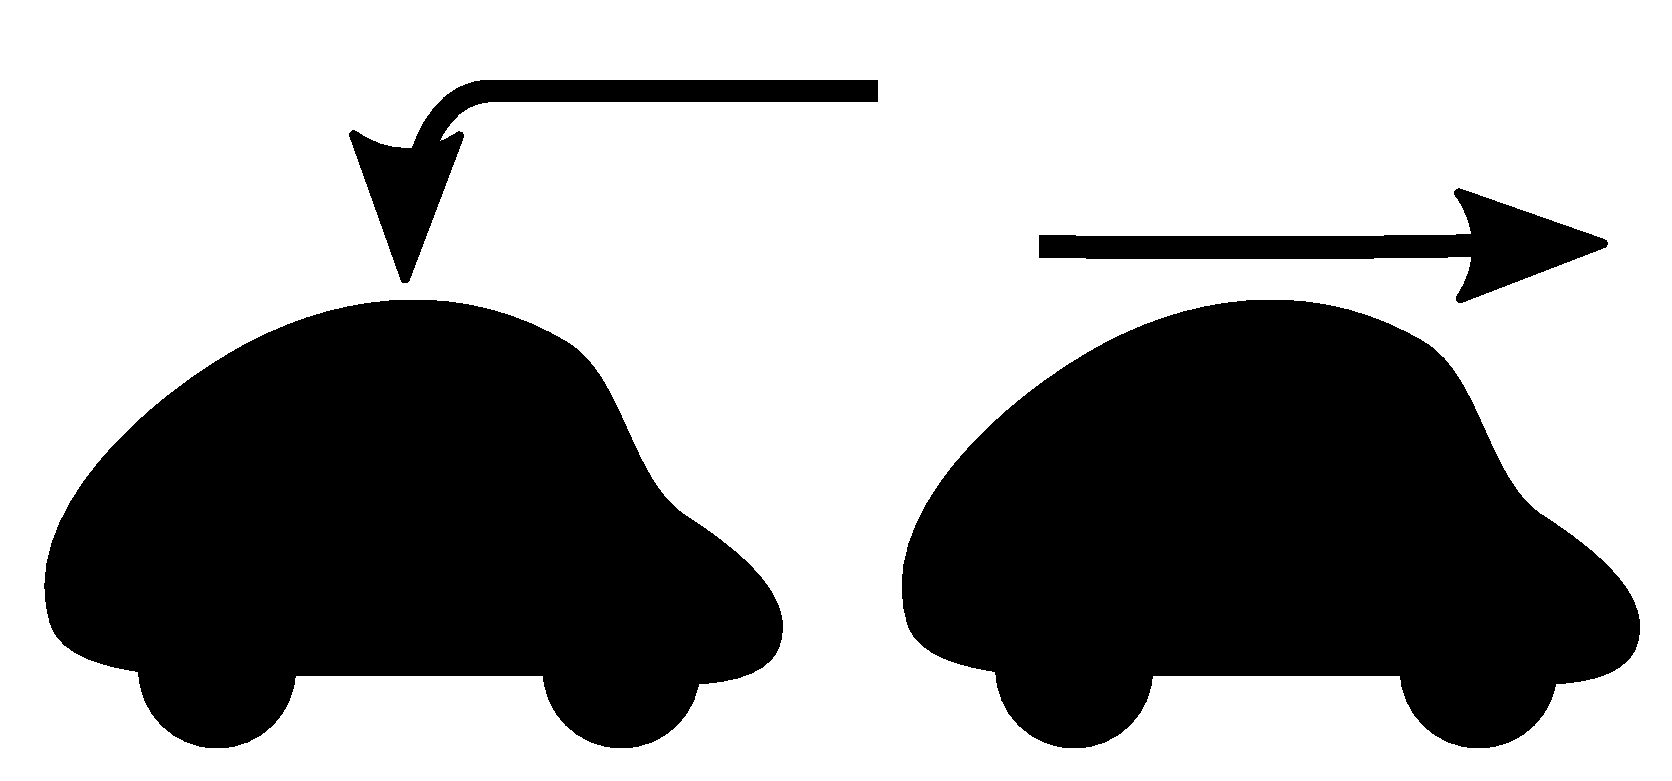
\includegraphics[height=30pt]{img/gaspedale/4.pdf}}}
	\newcommand{\symbolbild}{\raisebox{-.5ex}{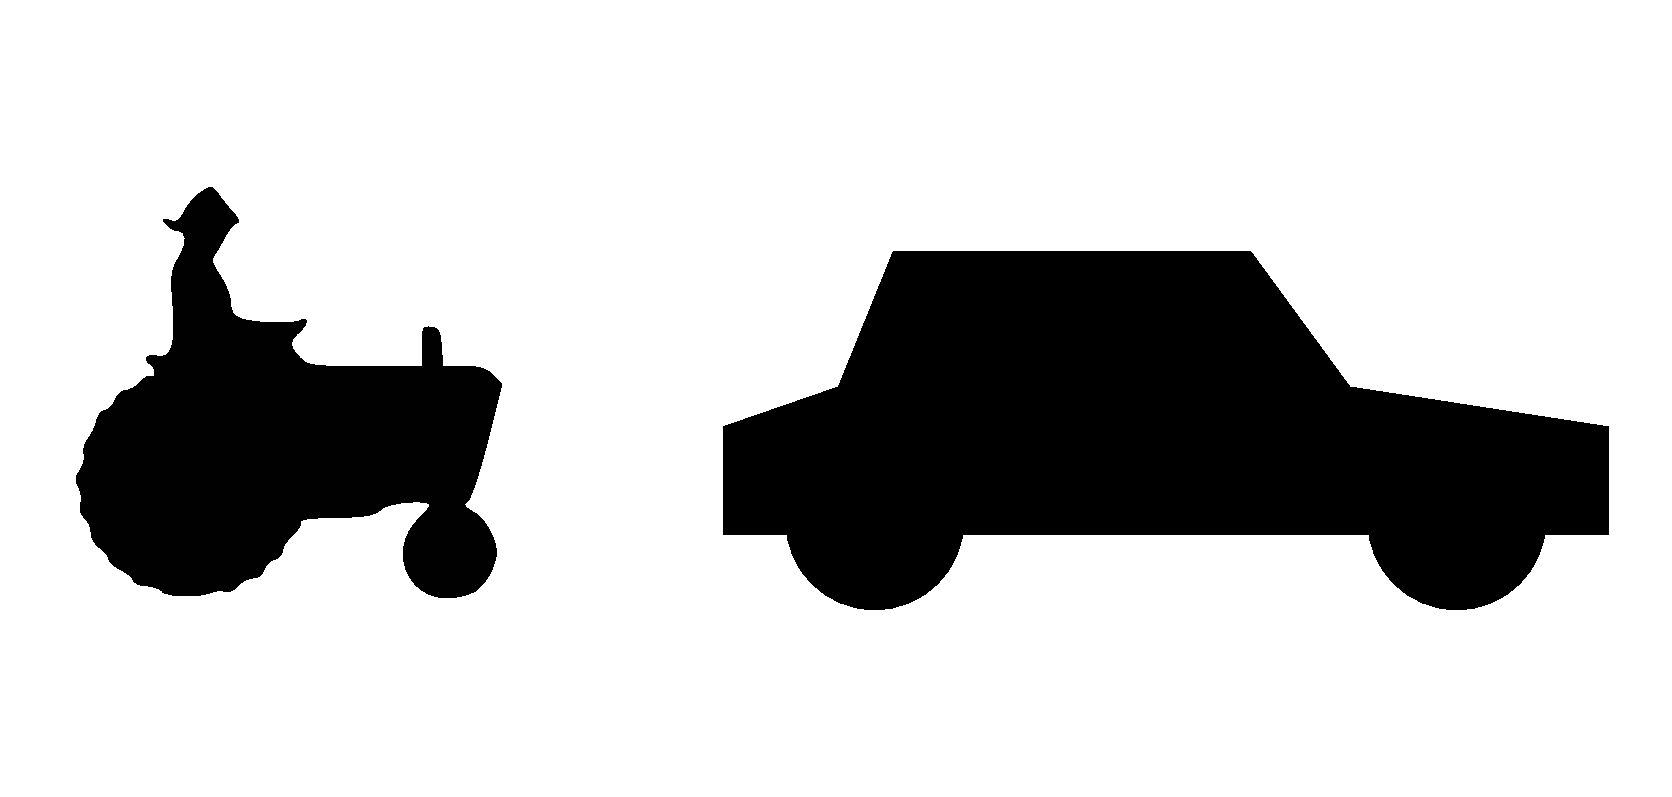
\includegraphics[height=30pt]{img/gaspedale/5.pdf}}}

	\begin{longtable}{cp{3.9cm}p{3.9cm}p{3.9cm}}%
		\toprule \endhead%
		\bottomrule \caption{Evolution der Pedale}\label{gasevo-tabelle} \endlastfoot%
			 & Beschreibung & Vorteile & Nachteile \\ \midrule
			\pedaleSchrift 		& Beschriftete Pedale werden in vielen Rennspielen verwendet. Dabei sind die Pedale mit \enquote{G} für Gas und \enquote{B} für Bremsen beschriftet. & Für deutschsprachige Spieler ist diese Einteilung einfach verständlich. & Im Rahmen der multilingualen Verwendbarkeit kann eine solche Beschriftung zu Missverständnissen führen. \\%
			\symbolbild 		& Eine weitere Möglichkeit ist die Verwendung von Symbolbildern. Dabei soll ein Symbol langsames Fahren und das andere schnelles Fahren symbolisieren. & Die Assoziation mit schnell und langsam ist sehr einfach. Die Symbole sind auch für Kinder sehr leicht verständlich. & Die Symbolbilder können nicht direkt als Schaltflächen erkannt werden. Eine Verwechslung mit beispielsweise einem Fahrzeugwechsel ist möglich und kann für Verwirrung sorgen.  \\%
			\autoPfeil 			&  Die Fahrzeuge werden mit entsprechenden erklärenden Pfeilen ausgestattet. Ein Pfeil zeigt auf das Fahrzeug selbst, was einen Stillstand symbolisiert. Der zweite Pfeil zeigt vom Fahrzeug weg, was eine Beschleunigung symbolisieren soll. & Durch die Verwendung des gleichen Fahrzeugs ist eine Assoziation mit einem Fahrzeugwechsel ausgeschlossen. & Die Bedeutung der jeweiligen Pfeile ist nicht eindeutig. Ein großer Interpretationsspielraum kann sehr leicht Missverständnisse hervorrufen. \\%
			\tacho 				& Zur Symbolisierung für schnelles und langsames Fahren werden Tachos mit unterschiedlichen Nadelausschlägen verwendet. Ein voll ausgeschlagener Tacho bedeutet dabei schnelles Fahren. & Da keine irritierenden Pfeile verwendet werden, sinkt die Gefahr eines Missverständnisses. Da ebenso kein Fahrzeug symbolisiert wird, kann auch jegliches Missverständnis in dieser Richtung vermieden werden. & Tachos sind leicht verwechselbar mit einer Benzinanzeige oder einer reinen Geschwindigkeitsanzeige. Usertests haben gezeigt, das Spieler nicht intuitiv auf die Tachos drücken. \\%
			\pedaleRealistisch 	& Das finale Design geht zurück zu den Pedalen, verzichtet jedoch auf die Beschriftung. Zur besseren Unterscheidbarkeit werden unterschiedliche Designs für die jeweiligen Pedale gewählt. Dabei orientieren sich die Pedale an Pedale von realen Fahrzeugen. & Die Pedale sind einfach als Schaltflächen erkennbar, durch das Verzichten auf Beschriftung sind die Pedale multilingual einsetzbar. Durch die Orientierung an realen Pedalen ist eine Assoziation mit diesen gegeben. & Der Spieler erkennt zwar nicht auf den ersten Blick, welche Funktion die Schaltflächen haben, kann dies jedoch über \enquote{Ausprobieren} testen. \\%
	\end{longtable}
	Der letzte Punkt im Bereich des UI Designs befasst sich mit der grundsätzlichen Positionierung der Schaltflächen und Icons. Wie in <TODO: Verlinkung zum Konzept> bereits erwähnt, soll das Spiel auf mobilen Endgeräten im Querformat gespielt und mit zwei Händen bedient werden. Da die wichtigsten Steuerelemente der Joystick sowie die Pedale sind, werden diese in den unteren Ecken zur Bedienung mit beiden Daumen positioniert. Die Schaltflächen für Pause und Zurücksetzen sind in den oberen Ecken positioniert, um eine versehentliche Betätigung durch den Spieler zu verhindern.
	\figur{Positionierung-UI.png}{\label{ssec:ui-design}User Interface mit geöffnetem Menü}
	Die Abbildung \ref{ssec:ui-design} zeigt das User Interface, während das Menü geöffnet ist. Die Menü-Schaltflächen für \enquote{Spiel fortsetzen / Spiel starten}, \enquote{Optionsmenü öffnen} sowie \enquote{Zum Hauptmenü zurückkehren} sind an der Mitte des Bildschirms orientiert.
	\figur{Positionierung-UI-2.png}{\label{ssec:ui-design2}User Interface während des Rennens}
	Während des Spiels entspricht das User Interface der Abbildung \ref{ssec:ui-design2}. An Stelle der Schaltflächen des Menüs befinden sich am oberen Bildschirmrand nun eine Zeitanzeige, sowie eine Minikarte. Die Minikarte stellt den Streckenverlauf leicht transparent dar und zeigt die Position und Rotation des Fahrzeugs mittels eines roten Pfeils an. Die Zeitanzeige ist als Zeitstrahl dargestellt. Dabei sinkt die Größe des gelben Anteils des Zeitstrahls. Ist kein gelber Anteil mehr vorhanden, so ist die Zeit für das Rennen vollständig abgelaufen.

	\subsubsection{Umsetzung der Steuerung}
	\lstset{language=[Sharp]C, % Grundsprache ist C und Dialekt ist Sharp (C#) c
	captionpos=b, % Beschriftung ist unterhalb
	frame=lines, % Oberhalb und unterhalb des Listings ist eine Linie
	basicstyle=\ttfamily, % Schriftart
	keywordstyle=\color{blue}, % Farbe für die Keywords wie public, void, object u.s.w.
	commentstyle=\color{green}, % Farbe der Kommentare
	stringstyle=\color{red}, % Farbe der Zeichenketten
	numbers=left, % Zeilennummern links vom Code
	numberstyle=\tiny, % kleine Zeilennummern
	numbersep=5pt, breaklines=true, % Wordwrap a.k.a. Zeilenumbruch aktiviert
	showstringspaces=false, % emph legt Farben für bestimmte Wörter manuell fest
	 emph={double,bool,int,unsigned,char,true,false,void}, emphstyle=\color{blue}, emph={Assert,Test}, emphstyle=\color{red}, emph={[2]\using,\#define,\#ifdef,\#endif}, emphstyle={[2]\color{blue}}}
	Die Steuerung des Fahrzeugs ergibt sich aus dem Zusammenspiel vieler Komponenten und Code-Bestandteile, welche über mehrere Skripte verteilt sind. In diesem Kapitel werden aus diesem Grund lediglich die wichtigsten Kernaspekte der Steuerung erläutert. Der Prozess der Steuerung läuft dabei in mehreren Schritten ab:
	\begin{enumerate}
		\item{ Das \enquote{CarUserControl} Skript entscheidet, ob das Fahrzeug fahren darf.}
		\item{ Falls ja erteilt das Skript dem \enquote{CarController} Skript den Befehl zur Bewegung}
		\item{ Im CarController wird die Ausrichtung des Joysticks ausgelesen.}
		\item{ Im CarController wird berechnet, um wieviel Grad das Fahrzeug drehen muss, um den gewünschten Winkel zu erhalten.}
		\item{ Die Räder werden im entsprechenden Winkel gedreht und das Fahrzeug bewegt sich in diese Richtung.}
	\end{enumerate}
	Im Folgenden sollen diese Schritte genauer analysiert werden. Dabei wird die Nummerierung aus der Aufzählung als Referenz verwendet.
	\begin{lstlisting}
private void FixedUpdate(){
[...]
//Überprüfe ob sich das Fahrzeug bewegen darf
  if (car.canMove){
    //Übermittle Befehl zur Bewegung
    m_Car.Move([...]]);
  }
}
	\end{lstlisting}
	Im CarUserControl Skripts aus Schtitt 1 wird regelmäßig die FixedUpdate() Methode ausgeführt. Regelmäßig bedeutet in diesem Fall eine Ausführung für jedes auf dem Bildschirm angezeigte Bild. Ob das Fahrzeug fahren darf, ist vom derzeitigen Status des \enquote{RaceController} Skripts abhängig. Der RaceController ist die Haupt-Kontrollinstanz für jedes gefahrene Rennen. Befindet sich der Spieler im Hauptmenü, so darf das Fahrzeug beispielsweise nicht fahren. In dem Moment, in welchem der Countdown vor einem Rennen abläuft, wird die Variable \enquote{canMove} auf \emph{true} gesetzt und das Fahrzeug darf losfahren. In diesem Moment übergibt die CarUserControl den Befehl zur Bewegung an den CarController.

	\begin{lstlisting}
public void Move([...]){
[...]
//Berechne Richtungsvektor des Joysticks
Vector3 direction =
  CrossPlatform.GetAxis("Vertical") * -Vector3.right
  + CrossPlatform.GetAxis("Horizontal") * Vector3.forward;
//Berechne den Drehwinkel zwischen aktueller Rotation des Fahrzeugs und der gewünschten Ausrichtung
Quaternion rotation = Quaternion.FromToRotation(
	(transform.rotation * Vector3.forward), direction);
	\end{lstlisting}

	Im nächsten Schritt wertet der CarController die Eingaben des Joysticks aus. Dazu greift er auf die Informationen des CrossPlatformInputManagers (im Codebeispiel als CrossPlatform abgekürzt) zurück. Dieser liefert Informationen über die horizontale und vertikale Ausrichtung des Joysticks. Dies sind generell Werte zwischen $-1$ und $1$. Durch Vektormultiplikationen mit den beiden Einheitsvektoren (x- und y-Richtung) entsteht ein Richtungsvektor. Dieser Richtungsvektor ist zweidimensional (bzw. der z-Wert ist immer $0$) und stellt die Zugrichtung des Joysticks dar.
	Aus der derzeitigen Ausrichtung des Fahrzeugs und dem zuvor errechneten Richtungsvektor kann eine Quaternion errechnet werden. Eine Quaternion beschreibt eine Bewegung eines Objekts. Die errechnete Quaternion beschreibt somit eine Rotation des Objekts von der derzeitigen Ausrichtung hin zur gewünschten Ausrichtung.

	\begin{lstlisting}
//Berechne Drehwinkel der Vorderräder
bool forwards = true;
steerAngle = rotation.eulerAngles.y;
if (180 - Mathf.Abs(steerAngle - 180) > m_MaximumSteerAngle){
  //Überprüfe, ob Fahrzeug rückwärts fährt
  if (steerAngle > 135 && steerAngle < 225){
	forwards = false;
	steerAngle = 360 - steerAngle;
	//Drehe Hinterräder um 180 Grad
	wheelCol[2].steerAngle = wheelCol[3].steerAngle = 180;
  } else {
    if (steerAngle >= 225){
	  steerAngle = 360 -m_MaximumSteerAngle;
    } else {
  	  steerAngle = m_MaximumSteerAngle;
    }
  wheelCol[2].steerAngle = wheelCol[3].steerAngle = 0;
  }
}
	\end{lstlisting}

	Im letzten Schritt müssen die Räder des Fahrzeugs entsprechend ausgerichtet werden. Dabei wird zunächst aus der Rotation ein Drehwinkel berechnet. Über die Fallunterscheidung aus dem Codebeispiel oben wird bestimmt, ob der Joystick entgegen der Fahrzeugausrichtung bewegt wird. Eine Bewegung entgegen der Ausrichtung des Fahrzeugs wird dabei als Befehl zum rückwärts fahren interpretiert. Um eine realistische Kurvenbahn zu erhalten, wird der Drehwinkel der Räder auf einen Bereich zwischen -45° und +45° begrenzt. Ein Bewegen des Joysticks außerhalb dieses Bereichs setzt den Winkel auf das jeweilige Maximum fest. So wird beispielsweise -60° in -45° umgewandelt. Somit ist gewährleistet, dass das Fahrzeug konstante Kurven fährt und das Angleichen der Fahrtrichtung an die Position des Joysticks nicht zu ruckartig geschieht. Das Verhalten der Räder bei Einschlagen des Rückwärtsgangs stellt eine Besonderheit dar. Die Räder sind mit einer Rotationsrichtung versehen, welche nicht einfach invertiert werden kann. Aus diesem Grund müssen alle Räder vollständig invertiert werden, wenn der Nutzer das Fahrzeug rückwärts steuern möchte. Die Hinterräder werden in diesem Fall exakt um 180° gedreht, die Vorderräder werden erst auf Basis des Lenkwinkels ausgerichtet und dann um 180° rotiert. Sobald die Fahrtrichtung wieder auf vorwärts wechselt, werden alle Räder erneut invertiert.

	Zur Realisierung der Beschleunigung ist eine Betrachtung des Rückwärtsgangs somit nicht nötig. Für die Beschleunigung wird eine zusätzliche Achse \enquote{Acceleration} entwickelt, welche mit dem Gaspedal verknüpft wird. Ein Betätigen des Gaspedals setzt den Wert der Achse auf 1, im generellen Fall beträgt der Wert 0. Das Bremspedal ist auf sehr ähnliche Weise definiert, ein Betätigen des Pedals setzt einen Wert \enquote{Bremskraft}, welcher ebenso wie die Beschleunigung in die generelle Bewegungsfunktion des Fahrzeugs eingebunden ist.


	\subsubsection{Physik}
	Im Rahmen dieser Arbeit wird auf die Entwicklung einer eigenen Physiksimulation verzichtet. Für die Implementierung der physikalisch interagierbaren Objekte wird auf die Grundfunktionen der Unity Engine zurückgegriffen. So können Objekte mit sogenannten \enquote{Physical Materials} versehen werden. Über diese Physical Materials können Objekte beispielsweise eine gewisse Elastizität erreichen oder wie Gummibälle von Gegenständen und Wänden abprallen. Über die Physical Materials wird versucht, die Reaktion der Objekte der Realität anzupassen. Die Leitkegel erhalten dabei einen höheren \enquote{Bouncyness} Wert als die Fässer, was dazu führt, das Leitkegel eher vom Fahrzeug abprallen, wohingegen Fässer eher vom Fahrzeug verschoben werden. Dieses Verhalten wird durch den erhöhten Gewichtswert der Fässer verstärkt, welcher dazu führt, dass die Fässer das Fahrzeug stärker abbremsen.

	\subsubsection{Verlangsamung des Fahrzeugs}
	\begin{lstlisting}
public void adjustTopSpeed()
{
float changeFactor = -Mathf.Cos(m_Topspeed/80 - 0.2f)*1.5f+1.6f;
if (isSlow){
    m_Topspeed = Mathf.Max(m_Topspeed - changeFactor * 1.3f, m_TopspeedSlow);
}else{
    m_Topspeed = Mathf.Min(m_Topspeed + changeFactor, m_TopspeedNormal);
}
}
    \end{lstlisting}
    Das Codebeispiel oben zeigt die beiden mathematischen Funktionen, welche für die Verlangsamung des Fahrzeugs verantwortlich sind. Der Methodenaufruf der adjustTopSpeed() Methode geschieht immer dann, wenn das Fahrzeug eine Zone betritt oder verlässt, welche die Geschwindigkeit manipuliert. Beim Betreten einer so genannten \enquote{SlowDown}-Zone wird die Variable \enquote{isSlow} auf \enquote{true} gesetzt. Daraufhin wird die Höchstgeschwindigkeit des Fahrzeugs kontinuierlich reduziert, bis die festgesetzte Geschwindigkeit erreicht ist. Verlässt das Fahrzeug die SlowDown-Zone wieder, so wird isSlow auf \enquote{false} gesetzt und die Höchstgeschwindigkeit des Fahrzeugs wird kontinuierlich erhöht, bis die ursprüngliche Höchstgeschwindigkeit erreicht ist.

	\subsubsection{Erkennung einer Frontalkollision}
	Um die Erkennung einer Frontalkollision zu ermöglichen, wird das Fahrzeug mit zwei Hilfs-Punkten ausgestattet. Diese Punkte sind jeweils mittig des Fahrzeugs positioniert, wobei eine der Punkte am vorderen Ende des Fahrzeugs und der zweite Punkt am Heck positioniert ist.
	\begin{lstlisting}
private void OnCollisionEnter(Collision collision){
Vector3 localAverageVorn = frontColliderHelper.transform.InverseTransformPoint(collision.contacts[0].point);
float distVorn = Vector3.Distance(localAverageVorn, new Vector3(0, 0, 0));
Vector3 localAverageBack = backColliderHelper.transform.InverseTransformPoint(collision.contacts[0].point);
float distBack = Vector3.Distance(localAverageBack, new Vector3(0, 0, 0));
if (distVorn <= 0.8 || distBack <= 0.8)
{
float speed = collision.relativeVelocity.magnitude;
float volume = Mathf.Pow(Mathf.Clamp(speed/10, 0f, 1f), 3);
GetComponent<NewGameAudio>().playCrashSound(volume);
}
}
\end{lstlisting}
	Das gezeigte Skript ist eine Komponente des Fahrzeugs. Im Moment der Kollision werden alle relevanten Daten über das kollidierte Objekt in einem Kollisions-Objekt gespeichert. Aus der Kollision können die Kontaktpunkte der beiden Objekte ausgelesen werden. Im nächsten Schritt wird die Durchschnittsposition aller Kontaktpunkte (also der mittlere aller Punkte) mit beiden eingangs erwähnten Hilfs-Punkten vergleichen. Dabei werden die derzeitigen Weltkoordinaten beider Punkte verwendet und die Distanz dieser beiden Punkte errechnet. Ist einer der beiden errechnet Werte (\enquote{distVorn} oder \enquote{distBack}) kleiner oder gleich 0.8, so wird von einer Frontalkollision ausgegangen. Der Abstand von 0.8 ist so gewählt, dass die äußeren Ecken des Fahrzeugs noch als Frontalkollision erkannt werden, seitlich versetzte Kollisionen jedoch nicht. Somit kann für beide Fälle ein anderer Sound abgespielt werden. Im Fall einer Frontalkollision wird ein Aufprall-Sound abgespielt, bei einer seitlichen Kollision ertönt ein \enquote{Kratzen}.
	Die Lautstärke des abgespielten Tons errechnet sich dabei aus der Geschwindigkeit des Fahrzeugs zum Zeitpunkt der Kollision. Je schneller das Fahrzeug mit einem Objekt kollidiert, desto lauter wird der Sound abgespielt.

	\subsubsection{Speicherung der Spielstände\label{speicherung}}
	Für die Speicherung der Spielstände stehen grundsätzlich zwei Möglichkeiten zur Verfügung. Zum einen kann eine Datenbank eingebunden werden, welche alle relevanten Daten speichert, zum anderen kann eine Datei erstellt werden, welche mittels serialisierbaren Feldern Informationen über den Spielfortschritt bereitstellt.
	Da keine großen Datenmengen zu erwarten sind, wird eine Datei im \enquote{.bin Format} verwendet.
	Die im Nutzerverzeichnis des Endgeräts befindliche \enquote{GameData.bin} enthält Informationen über die bereits gewonnenen Rennen, über freigeschaltete Gegenstände aus dem Shop, über die Anzahl an Münzen, die der Nutzer besitzt, sowie die aus dem Shop ausgerüsteten Gegenstände. Dadurch ist gewährleistet, dass der Nutzer das Spiel bei einem Neustart im gleichen Zustand vorfindet, wie es verlassen wurde.
	Alle genannten Attribute sind über sogenannte [SerializeField] Attribute definiert, was eine Speicherung im Textformat ermöglicht. Über den Aufruf \enquote{GameData.GetInstance()} kann an jeder beliebigen Stelle des Programmcodes auf die gespeicherten Werte zugegriffen werden. Somit ist eine Anwendungsweite Synchronisation gewährleistet.

	\subsubsection{Performance und Dateigröße}
	Ein wichtiger Schritt der Entwicklung des Spiels ist die Performance der Anwendung. Durch die Vorgaben der Aufgabenstellung soll das Spiel auch für Kinder der ärmeren Bevölkerungsschichten zugänglich sein. Kinder, die diesen Schichten angehören, besitzen häufig keine sehr guten mobilen Geräte. Somit rückt die Performance in den Vordergrund.
	Vor der Optimierung der Anwendung ist diese auf einem \emph{HTC ONE M8} gerade so spielbar. Die Anwendung ruckelt leicht, ein erfolgreiches Abschließen der Level ist jedoch ohne weiteres möglich. Auf dem zweiten Testgerät, einem \emph{Samsung Galaxy S2} sowie auf dem \emph{Fairphone 2} ist die Anwendung unspielbar und springt langsam von einem Standbild zum nächsten.
	Hinzu kommt, dass die Anwendung in diesem Status der Entwicklung zu viel Speicherplatz einnimmt. Vor der Optimierung beträgt die Größe der APK-Installationsdatei ca $100$ MB, das installierte Spiel nimmt $280$ MB ein.

	Für die Optimierung der Performance und der Dateigröße werden folgende Schritte definiert:
	\begin{itemize}
	\item{ Reduzierung der Dateigröße durch höhere Kompression der Texturen.}
	\item{ Verbesserung der Performance durch geringere Qualitätseinstellungen für Texturen und 3D Modelle.}
	\item{ Optimierung der Performance durch entfernen einiger Elemente aus den Leveln.}
	\item{ Reduzierung der Dateigröße durch geringere Standardgröße aller 3D Objekte.}
	\end{itemize}

	Nach der Durchführung der vier genannten Schritte ist eine deutliche Optimierung sichtbar. Die Dateigröße der APK-Installationsdatei ist auf etwa $70$ MB gesunken, die Größe des installierten Spiels auf dem Endgerät beträgt lediglich noch $128$ MB.
	Auf dem \emph{HTC ONE M8} läuft die Anwendung merklich flüssiger, die leichten Ruckler sind kaum erkennbar. Auf dem \emph{Samsung Galaxy S2} konnte die Anwendung leider nicht flüssig ausgeführt werden. Die Bildrate ist durch die Optimierung merklich gestiegen, jedoch ist ein gut spielbarer Status nicht erreicht. Auf dem \emph{Fairphone 2} konnte die optimierte Anwendung bis zum aktuellen Zeitpunkt nicht erneut getestet werden.

	Die Verteilung der einzelnen Optimierungsschritte sieht dabei wie folgt aus:
	Die Reduzierung der Standardgröße aller 3D Objekt hat leider nicht den gewünschten Effekt erzielt. Die endgültige Dateigröße hat sich durch diesen Schritt um lediglich $2$ MB verkleinert. Die höhere Kompression der Texturen hatte im Rahmen der Optimierung den größten Effekt. Die Größe aller Texturen konnte von insgesamt rund $240$ MB auf $20$ MB verringert werden. Diese Werte sind nicht direkt im obigen Gesamtergebnis erkennbar, da die Texturen im Laufe des Build-Prozesses erneut komprimiert werden.
	Im Rahmen der Performanceoptimierung konnte der größte Erfolg durch das Entfernen einiger Elemente aus den Leveln erzielt werden. Die geringeren Qualitätseinstellungen für Texturen und Modelle verändern hierbei lediglich die Optik, verändern jedoch die Performance nur minimal.

\subsection{Struktur und Aufbau}
Wie im vorherigen Kapitel bereits erwähnt, werden Programmfunktionen in Unity grundsätzlich über Skripte realisiert. Diese Skripte sind in den meisten Fällen unabhängig voneinander. Das Zusammenfügen der Komponenten wird in diesem Fall von der Unity Engine übernommen. Von einer Darstellung aller internen Komponenten der Engine wird an dieser Stelle abgesehen, da während der Entwicklung des Spiels kein Einfluss auf diese internen Verknüpfungen genommen werden kann. Da eine Darstellung der einzelnen Skripte lediglich eine Zusammenstellung von einzelnen Dateien ist und somit kein Mehrwert für die Arbeit erziehlt werden kann, wird dies ebenso unterlassen. Allgemein zusammengefasst lässt sich ableiten: Die Unity Engine steht in der Mitte eines Diagramms, viele Skripte sind in Form einer Wolke um die Engine verteilt, stehen jedoch nicht in Verbindung zueinander.
Bei der Implementierung des Spiels wurde keine Datenbank verwendet. Die Datenspeicherung geschieht wie in \ref{speicherung} bereits erwähnt über die Datei \enquote{GameData.bin}.

\subsection{Integration in Lernplattform}
	Die Integration in die Lernplattform von Incekara und Wolske\footcite{lernplattform} konnte nicht umgesetzt werden. Die Möglichkeiten des Spiels verschiedene Lernstandards gleichzeitig zu implementieren sind nicht in der Plattform vorgesehen und es müsste eine Schnittstelle implementiert werden.
	Eine Möglichkeit diese Schnittstelle umzusetzen wurde ausgearbeitet aber schlussendlich nicht verwendet.
	\subsubsection*{Beschreibung Schnittstelle}
		Für die Kommunikation zwischen Anwendungen auf Android ist die Verwendung von AIDL\footcite{android-interfaces} oder ähnlichem nötig.\footnote{Weitere Möglichkeiten werden auf der zitieren Seite genannt.}
		Ein unterstütztes Lernspiel bietet zwei Schnittstellen:
		\begin{description}
			\item[Lernstandards auflisten]{
				Gibt eine Liste der unterstützten Standards zurück.
			}
			\item[Mit Standard $X$ starten]{
				Startet das Spiel mit dem ausgewähltem Standard.
			}
		\end{description}
		Für die Lernplattform reicht es aus die Standards beim Starten für alle Spiele zu sammeln und wenn vom Spieler gewünscht diese mit dem Passendem Standard starten.

% !TEX root = dokumentation.tex
\section{Evaluation}
	Was lief nicht

	Was lief anders
\subsection{Requirements Analyse}
\subsection{Lernziele evaluation}
\subsection{Testversuch mit Kind?}
	\begin{enumerate}
		\item{ matheaufgabe - 1 woche spielen - noch ne mathe aufgabe }
		\item{ spaßfaktor? }
		\item{ feedback durch eltern }
	\end{enumerate}

% !TEX root = dokumentation.tex
\section{Zusammenfassung}
\subsection{Fazit}
\subsection{Ausblick}

\pagebreak
\nocite{*}
\printbibliography
\pagebreak
%% !TEX root = projectmanagement.tex

\section{Anhang}
\pagebreak
\subsection*{Gesprächsprotokolle}
% !TEX root = Projektmanagement/projectmanagement.tex
\textbf{Kickoff-Meeting:} (2016-11-03)\\
Folgende Fragen waren vorbereitet, um sie Prof. PhD. Kay Berkling zu stellen:
\begin{itemize}
	\item Welche Anforderung müssen wir für Note 1 erfüllen?
	\item Welche Zielvoraussetzungen sind für das Spiel gesetzt?
	\item Für wieviel Spielzeit soll das Spiel den Spieler unterhalten?
	\item Für welche Altersklasse soll das Spiel sein?
	\item Welche Art Lernmöglichkeit soll implementiert werden?
	\item Sind die Lernstandards einzuhalten?
\end{itemize}

Auf Basis dieser Fragen konnten folgende Grundsätze für die Studienarbeit festgelegt werden:
\begin{enumerate}
	\item Die Bewertung der Studienarbeit wird anhand des Excel-Sheets zur Bewertung von Praxis-, Bachelor- und Studienarbeiten durchgeführt.
	\item Das Layout sowie die Outline der Studienarbeit und der Terminplan sind vorher mit Prof. PhD. Kay Berkling zu besprechen.
	\item Die exakten Kriterien für die Erfüllung der Anforderungen befindet sich auf der eigens dafür eingerichteten Seite \enquote{http://dhbwstudienarbeit.pbworks.com/}.
	\item Um sicherzustellen, dass die Studienarbeit im gesetzten Zeitrahmen erfolgreich abgeschlossen wird, sollen bis zum 15. Januar bereits 80\% des Textes verfasst sein. Die Evaluation über den Erfolg der Arbeit stellt die fehlenden 20\%.
	\item Die fertige Studienarbeit ist 4 Wochen vor dem eigentlichen Endtermin (also am 17.04.2017) vollständig bei Prof. PhD. Kay Berkling abzugeben.
	\item Beim Inhalt der Studienarbeit ist auf Wissenschaftlichkeit zu achten. Zum Belegen von Thesen etc. ist eine Bibliographie von min. zwei Seiten zu liefern.
	\item Es besteht keine Notwendigkeit der Einhaltung der Lernstandards. Die Spieler (Kinder) sollen mit dem Spiel Spaß haben und das Spiel auch spielen \enquote{wollen}.
	\item Die Zielgruppe für das Lernspiel besteht aus Kindern im Alter der ersten bis sechsten Klasse. Nach Möglichkeit soll dieses Spiel und die zugehörige Lernplattform auch Flüchtlingskindern zur Verfügung gestellt werden.
	\item Als Beispiele zur Orientierung wurde \enquote{arcademics.com} genannt, welche Spiele der gewünschten Art beinhaltet, jedoch eine Internetverbindung benötigt. Daraus ergibt sich, dass das Spiel auch offline spielbar sein soll.
\end{enumerate}




% !TEX root = Projektmanagement/projectmanagement.tex
\textbf{Mehrere Brainstorming-Sessions:} (Themenbekanntgabe bis 2016-11-03)\\
In mehreren kleinen Brainstorming-Sessions zwischen den beiden Bearbeitern der Studienarbeit, welche noch vor dem Kickoff-Meeting abgehalten wurden, konnten diverse Grundsätze festgesetzt werden:
\begin{itemize}
	\item min 2h Spielspaß
	\item educational game: Nicht offensichtlich ein Lernspiel
	\item Programmieraufwand: drei Monate (all inclusive)
	\item casual game
	\item originelle Idee (kein Klon)
	\item offline spielbar
	\item kein RPG im engeren Sinne
\end{itemize}

Folgende Ideen zu Spielen wurden in weiteren Brainstorming-Sessions erarbeitet:
\begin{enumerate}
	\item Chemie / Physik Simulation:
	\begin{itemize}
		\item Laborumgebung
		\item Einfache Experimente durchführbar
		\item Fehler in Experimenten führt zu scheitern
		\item Steuerung der Hände des Laborarbeiters
		\item Idee wegen schwerer Durchführbarkeit (Partikelsystem etc) sowie geringem Lernerfolg verworfen
	\end{itemize}
	\item Rätselspiel:
	\begin{itemize}
		\item Aufgrund fehlernder weiterer Eingebung verworfen
	\end{itemize}
	\item Simulation von Motoren und Getrieben
	\begin{itemize}
		\item Spieler bekommt zu fahrende Strecke gezeigt (2D Ansicht)
		\item Auswahl verschiedener Motoren möglich
		\item Auswahl des Treibstoffes möglich
		\item Gangschaltung während der Fahrt möglich
		\item Informationstexte über Motoren sowie Treibstoffe und Übersetzungen der Zahnräder
		\item Zeitrennen / Erreichen des Ziels als Spielziel
		\item Idee nach dem Kickoff-Meeting vollständig verworfen aufgrund unpassender Lernumsetzung
	\end{itemize}
	\newpage
	\item Rennfahrspiel mit Verkehrsregelaufgaben und Mini Aufgaben:
	\begin{itemize}
		\item wilde renntour durch die stadt
		\item Polizeiverfolgung und verschiedenen Animationen des Scheiterns (Death Sells)
		\item zu lösende Aufgabe bei jedem Scheitern
		\item Minigame mit verschiedenen aufgaben wie:
		\begin{itemize}
			\item ampel: es muss gebremst werden (mögliche Fail Animationen, fährt in ein Auto rein, bleibt stehen aber explodiert, fährt die Ampel um)
			\item Polizei: es muss rechts rangefahren werden
			\item Sprungschantze: Gas geben statt bremsen
			\item Kurven links / rechts
		\end{itemize}
		\item Nach dem Kickoff-Meeting verworfen
	\end{itemize}
\end{enumerate}


\textbf{Erstes Team-Meeting:} (2016-11-06)\\
Nach dem Kickoff-Meeting und der genauen Definiton der Anforderungen und Wünsche konnte eine genaue Spielidee entwickelt werden.
Das Ergebnis des Team-Meetings ist die zu Anfang erwähnte Spielidee, welche maßgeblich durch die vorherigen Ideen der Brainstorming-Sessions beeinflusst wurde. Dabei wurden die Ergebnisse dieser Sessions zusammengefasst und auf das gewünschte gefiltert.
\newline
% !TEX root = Projektmanagement/projectmanagement.tex
gamifaction kein modell raussuchen,
	persona definieren, gamification faktoren extrahieren
jira => youtrack
grundlagen neusortiert
Gameengines
spieleidee abesprochen - gut
um models kümmern (kassenschluss ende november)
inhaltsverzeichnis abgesprochen - gut

% !TEX root = Projektmanagement/projectmanagement.tex
\textbf{Zweites Teammeeting:} (2016-11-17)\\
Die Tagesordnung für das zweite Teammeeting bestand aus folgenden Punkten:
\begin{itemize}
	\item{Verfassen eines aussagekräftigen Titels}
	\item{Verfassen von Requirements und Usecases}
	\item{Vorauswahl von Game-Engines}
	\item{Heraussuchen von Models und Grafiken}
\end{itemize}

Zum Verfassen des Titels wurden zunächst mehrere Möglichkeiten gesammelt:
\begin{itemize}
	\item{Konzeption und Entwicklung eines Computerspiels um Schulwissen spielerisch zu lehren}
	\item{Schulwissen lernen durch ein Android basiertes Spiel}
	\item{Vermittlung von Schulwissen durch ein Android Spiel}
	\item{Vermittlung von Schulwissen durch spielerisches lernen auf Android}
	\item{Spielerisch Schulwissen vermitteln auf Android - Konzeption und Entwicklung eines educational games}
	\item{Konzeption und Entwicklung eines educational games - Spielerisch Schulwissen vermitteln auf Android}
\end{itemize}
Der zuletzt genannte Titel hat dabei den besten Anklang bei beiden Teammitgliedern gefunden, daher wurder er als finaler Titel gewählt.

Bezüglich der Models und Grafiken wurd beschlossen, einen externen Grafiker für die Gestaltung der Spielwelt hinzuzuziehen. Weiterhin sollen Models verwendet werden, welche bereits im Besitz der DHBW sind um die entstehenden Kosten so gering wie möglich zu halten.
Daraufhin wurde eine Nachricht an einen entsprechenden Grafiker verfasst, welcher den Auftrag angenommen hat. Dieser wird bei Zeiten einige Skizzen einreichen, aus welchen das fertige Spieldesign gewählt werden soll.

Die Punkte \enquote{Verfassen von Requirements und Usecases}, sowie \enquote{Vorauswahl der Game-Engines} wurden aus Zeitgründen vertagt.


\end{document}